\documentclass[fleqn]{beamer}

\usepackage[british]{babel}
\usepackage{graphicx,ru,url}
\usepackage{amsmath}
% Use Times for math font and text font.
\RequirePackage[T1]{fontenc}
%\RequirePackage{txfonts}
% bold math must be loaded after Times font
\usepackage{bm}
\usepackage{booktabs} % nice rules (thick lines) for tables
\usepackage{microtype} % improves typography for PDF
\usepackage{xcolor}
\usepackage{tikz}
\usepackage{verbatim}
\usetikzlibrary{arrows,shapes,snakes}
\usepackage{hyperref}

\graphicspath{{figures/}} % Specifies the directory where pictures are stored

% The title of the presentation:
%  - first a short version which is visible at the bottom of each slide;
%  - second the full title shown on the title slide;
\title[Energy Expansion using KLT]{
  Energy Expansion in Response Matrix Methods Using the Karhunen-Lo\`{e}ve Transform}

% Optional: a subtitle to be displayed on the title slide
%\subtitle{Show where you're from}

% The author(s) of the presentation:
%  - again first a short version to be displayed at the bottom;
%  - next the full list of authors, which may include contact information;
\author[Richard Reed]{
  Richard Reed \\
  Dr. Jeremy Roberts}

% The institute:
%  - to start the name of the university as displayed on the top of each slide
%    this can be adjusted such that you can also create a Dutch version
%  - next the institute information as displayed on the title slide
\institute[Kansas State University]{
  Mechanical and Nuclear Engineering \\
  Kansas State University}

% Add a date and possibly the name of the event to the slides
%  - again first a short version to be shown at the bottom of each slide
%  - second the full date and event name for the title slide
\date[2014 ANS Annual Meeting]{
  2014 ANS Annual Meeting \\
  18th June 2014}

\begin{document}
  %\renewcommand*{\inserttotalframenumber}{\pageref{lastframe}}
  \newcommand{\beginbackup}{
    \newcounter{framenumbervorappendix}
    \setcounter{framenumbervorappendix}{\value{framenumber}}
  }
  \newcommand{\backupend}{
    \addtocounter{framenumbervorappendix}{-\value{framenumber}}
    \addtocounter{framenumber}{\value{framenumbervorappendix}}
  }

  \begin{frame}
    \titlepage
  \end{frame}

  \begin{frame}
    \frametitle{Outline}
    \begin{block}{Presentation Outline}
      \begin{itemize}
	\item Introduction and Background
	\begin{itemize}
	  \item Response Matrix Method
	  \item Energy Expansion
	\end{itemize}
	\item Test Problems and Models
	\begin{itemize}
	  \item 10-Pin Test Problem
	  \item BWR Test Problem
	\end{itemize}
	\item Results and Analysis
	\item Conclusion
      \end{itemize}
    \end{block}
  \end{frame}

  \section{Introduction and Background}

%  \begin{frame}
%    \frametitle{Introduction and Background}
%    \begin{block}{Section Outline}
%      \begin{itemize}
%	\item Response Matrix Method
%	\item Discrete Legendre Polynomials (DLP)
%	\item Modified DLP (mDLP)
%	\item Karhunen-Lo\`{e}ve Transform
%      \end{itemize}
%    \end{block}
%  \end{frame}

  \begin{frame}
    \frametitle{Response Matrix Method}
    \begin{columns}[c]
      \begin{column}{0.5\textwidth}
	\begin{block}{Overview}
	  \begin{itemize}
	    \item Breaks global domain into independent nodes
	    \item Nodes are linked by boundary conditions.
	    \item Boundary conditions based on truncated, orthogonal basis expansions
	    \item Sweep across nodes for global solution
	  \end{itemize}
	\end{block}
      \end{column}
      \begin{column}{0.5\textwidth}
	Reactor Eigenvalue Equation
	\begin{equation}
	  \mathcal{T} \phi(\bm{\rho}) = \frac{1}{k} \mathcal{F} \phi(\bm{\rho}) \, , \nonumber
	\end{equation}
	where $\bm{\rho}$ contains the relevant phase space (i.e., $\mathbf{r}$, $E$, and $\Omega$).
	\vspace{\baselineskip}

	Codes {\tt Serment} and {\tt Detran} used for calculations
      \end{column}
    \end{columns}
  \end{frame}

  \begin{frame}
    \frametitle{Expanding in Energy Groups}
    Energy Phase Space discretized by groups
    \begin{columns}[T]
      \begin{column}{0.5\textwidth}
	\begin{block}{Background}
	  \begin{itemize}
	    \item RMM typically uses few (<7) groups
	    \item More groups means greater fidelity
	    \item Fewer DOF mean faster computations
	  \end{itemize}
	\end{block}
      \end{column}
      \begin{column}{0.5\textwidth}
	\begin{block}{Goals}
	  \begin{itemize}
	    \item Reduce groups by order of magnitude
	    \item Achieve sub $0.1\%$ relative error in fission density
	  \end{itemize}
	\end{block}
      \end{column}
    \end{columns}
  \end{frame}


  \begin{frame}
    \frametitle{Modified Discrete Legendre Polynomials}
    \begin{columns}[T]
      \begin{column}{0.4\textwidth}
	\begin{block}{Creating mDLPs}
	  \begin{itemize}
	    \item Impose spatially averaged flux profile as $0^{th}$ order
	    \item Resulting polynomials are orthogonalized
	    \item Improves DLP by imparting relevant phase space information
	  \end{itemize}
	\end{block}
      \end{column}
      \begin{column}{0.6\textwidth}
	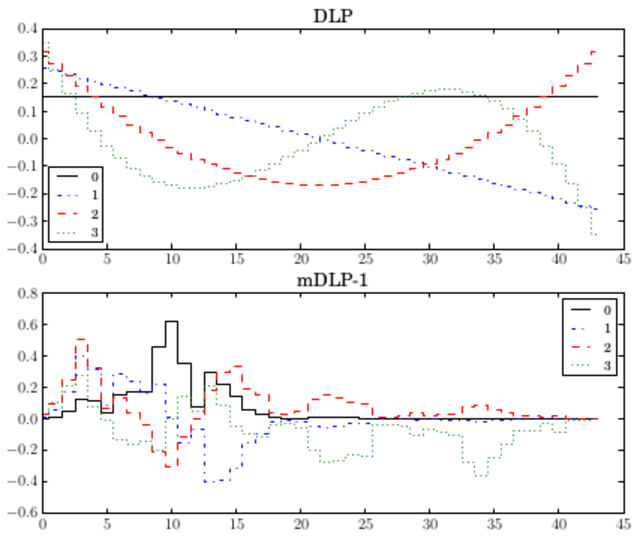
\includegraphics[totalheight=.65\textheight]{mDLP}
      \end{column}
    \end{columns}
  \end{frame}

  \begin{frame}
    \frametitle{Karhunen Lo\'{e}ve Transform}
    Form matrix $\mathbf{D}$ from snapshots of $\phi$ or other term of interest.
    \begin{columns}[c]
      \begin{column}{0.5\textwidth}
	$\mathbf{D}$ = \begin{bmatrix}
	  \phi_{1,1} & \phi_{1,2} & \cdots & \phi_{1,s} \\
	  \phi_{2,1} & \phi_{2,2} & \cdots & \phi_{2,s} \\
	  \vdots & \vdots & \ddots & \vdots \\
	  \phi_{g,1} & \phi_{g,2} & \cdots & \phi_{g,s}
	\end{bmatrix}
      \end{column}
      \begin{column}{0.5\textwidth}
	\setlength{\mathindent}{0pt}
	\begin{equation}
	  \mathbf{B} = \mathbf{D}^{T}\mathbf{D} \, \nonumber
	\end{equation}
	\begin{equation}
	  \mathbf{Bb}_j = \lambda_j \mathbf{b}_j \,  \quad \& \quad \lambda_j > \lambda_{j+1} \, , \forall j \, \nonumber
	\end{equation}
	\begin{equation}
	  \mathbf{y}_j = \mathbf{D}\mathbf{b}_j \, \nonumber
	\end{equation}
	\begin{equation}
	  \mathbf{f} \approx \sum_j a_j \mathbf{y}_j \, \quad \& \quad a_j = \mathbf{f}^T \mathbf{y}_j \, \nonumber
	\end{equation}
      \end{column}
    \end{columns}
    After orthogonalization of $\mathbf{y}_j$, transform generates a number of basis vectors equal to number snapshots (in this case, g).
  \end{frame}

  \section{Test Problems and Models}

%  \begin{frame}
%    \frametitle{Test Problems and Models}
%    \begin{block}{Section Outline}
%      \begin{itemize}
%	\item 10-pin Test Problem
%	\item 10-pin Snapshot Generation
%	\item BWR Test Problem
%	\item BWR Snapshot Generation
%      \end{itemize}
%    \end{block}
%  \end{frame}

  \begin{frame}
    \frametitle{10-pin Test Problem}
    \begin{block}{Pin Cell Mesh}
      \begin{itemize}
	\item 22 mesh cells of fuel
	\item 3 mesh cells of moderator on either side
	\item Each pin cell provides 28 energy-dependent snapshots
      \end{itemize}
    \end{block}
    \begin{center}
      \begin{figure}
	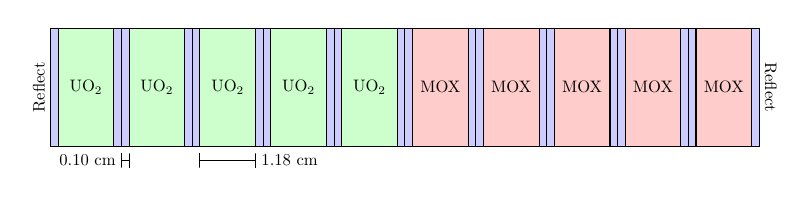
\begin{tikzpicture}[scale=0.6, every node/.style={scale=0.6}]
	  \foreach \x in {0,1.5,...,6}
	    \filldraw[xshift=\x cm, fill=green!20!white, draw=black] (0.160714286,0) rectangle (1.339285714,2.5) node[pos=.5] {UO$_2$};
	  \foreach \x in {7.5,9,...,13.5}
	    \filldraw[xshift=\x cm, fill=red!20!white, draw=black] (0.160714286,0) rectangle (1.339285714,2.5) node[pos=.5] {MOX};
	  \foreach \x in {0,1.5,...,13.5}
	    \filldraw[xshift=\x cm, fill=blue!20!white, draw=black] (0,0) rectangle (0.160714286,2.5);
	  \foreach \x in {0,1.5,...,13.5}
	    \filldraw[xshift=\x cm, fill=blue!20!white, draw=black] (1.339285714,0) rectangle (1.5,2.5);
	  \draw[xshift=15cm,yshift=1.25cm] node[right] {\rotatebox{-90}{Reflect}};
	  \draw[yshift=1.25cm] node[left] {\rotatebox{90}{Reflect}};
	  \draw (1.5,-.15) -- (1.5,-.45) -- (1.5,-.30) node[left] {0.10 cm} -- (1.660714286,-.30) -- (1.660714286,-.15) -- (1.660714286, -.45);
	  \draw (3.160714286,-.15) -- (3.160714286,-.45) -- (3.160714286,-.30) -- (4.339285714,-.30) node[right] {1.18 cm} -- (4.339285714,-.15) -- (4.339285714, -.45);
	\end{tikzpicture}
      \end{figure}
    \end{center}
    \begin{block}{Test Problem Settings}
      \begin{itemize}
	\item 16-angle, double Gauss-Legendre quadrature
	\item Step characteristics spatial discretization
      \end{itemize}
    \end{block}
  \end{frame}

  \begin{frame}
    \frametitle{10-pin Snapshot Generation}
    \begin{table}
      \begin{tabular}{l | p{7cm}}\toprule
	Abbreviation    & Model to generate snapshots \\
	\hline
	MOX Pin         & MOX pin only \\
	UO$_2$ Pin      & UO$_2$ pin only \\
	Combined Pins  & 1 UO$_2$ pin, 1 MOX pin, Pin Junction modeled separately then combined \\
	N pin           & Repeating array of N UO$_2$ and N MOX pin \\
	\bottomrule
      \end{tabular}
      \label{tab:snapshots}
    \end{table}
  \end{frame}

%  \begin{frame}
%    \frametitle{BWR Test Problem}
%    \begin{center}
%    Assemblies and pin cells had reflective conditions.

%    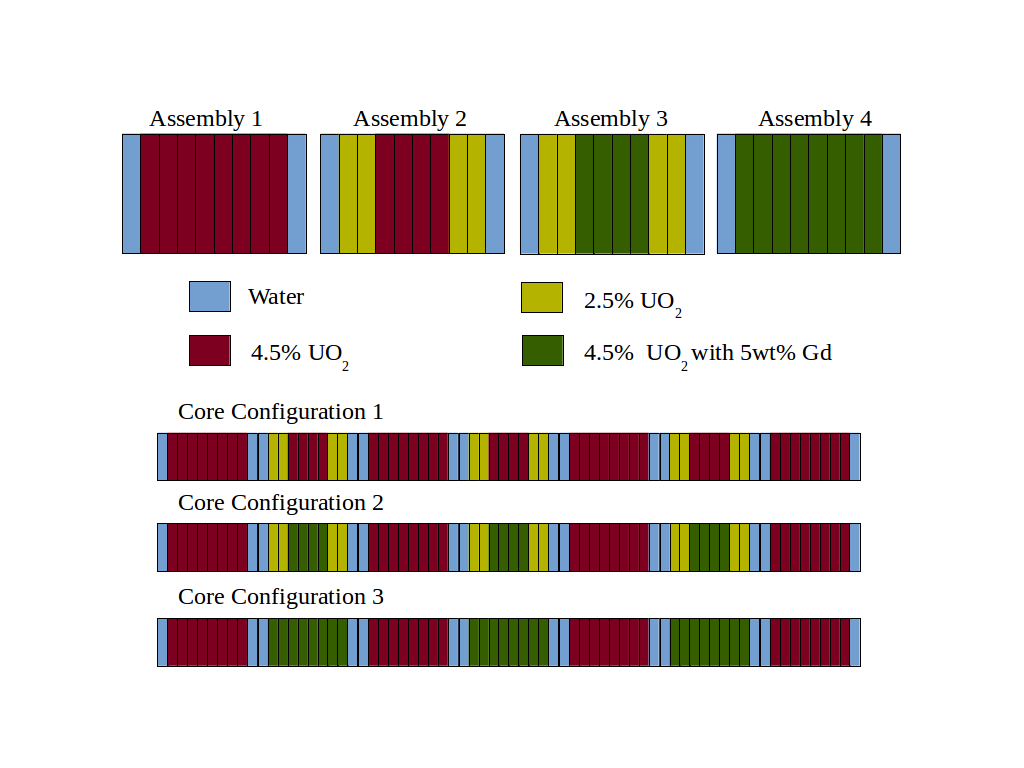
\includegraphics[trim=3.2cm 3.5cm 4.2cm 3.2cm, clip=true, totalheight=.7\textheight]{config}

%    Core models had vacuum boundary conditions.
%  \end{frame}

  \begin{frame}
    \frametitle{BWR Test Problem}
    \begin{center}
    Assemblies and pin cells had reflective conditions.

    \begin{figure}
      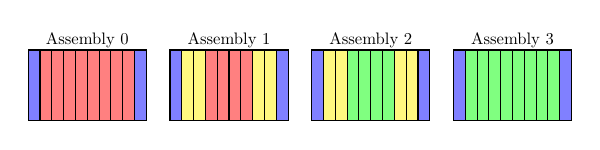
\begin{tikzpicture}[scale=0.6, every node/.style={scale=0.6}]
	\foreach \x in {0,2.25,3,5.25,6,8.25,9,11.25}
	  \filldraw[xshift=\x cm,fill=blue!50!white,draw=black] (0,0) rectangle (0.25,1.5);
	\foreach \x in {.25,.5,.75,1,1.25,1.5,1.75,2,3.75,4,4.25,4.5}
	  \filldraw[xshift=\x cm,fill=red!50!white,draw=black] (0,0) rectangle (0.25,1.5);
	\foreach \x in {3.25,3.5,4.75,5,6.25,6.5,7.75,8}
	  \filldraw[xshift=\x cm,fill=yellow!50!white,draw=black] (0,0) rectangle (0.25,1.5);
	\foreach \x in {6.75,7,7.25,7.5,9.25,9.5,9.75,10,10.25,10.5,10.75,11}
	  \filldraw[xshift=\x cm,fill=green!50!white,draw=black] (0,0) rectangle (0.25,1.5);
	\draw (0.25,1.7) node[right] {Assembly 0};%
	\draw (3.25,1.7) node[right] {Assembly 1};%
	\draw (6.25,1.7) node[right] {Assembly 2};%
	\draw (9.25,1.7) node[right] {Assembly 3};%
      \end{tikzpicture}
    \end{figure}
    \begin{figure}
      \vspace*{-.35cm}
      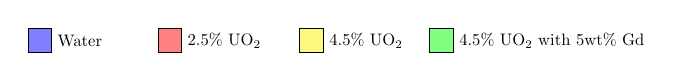
\begin{tikzpicture}[scale=0.6, every node/.style={scale=0.6}]
	\filldraw[xshift=-4cm,fill=blue!50!white,draw=black] (-.25,-.25) rectangle (.25,.25) node[yshift=-.25cm, right] {Water};%
	\filldraw[xshift=-1.25cm,fill=red!50!white,draw=black] (-.25,-.25) rectangle (.25,.25) node[yshift=-.25cm, right] {2.5$\%$ UO$_2$};%
	\filldraw[xshift=1.75cm,fill=yellow!50!white,draw=black] (-.25,-.25) rectangle (.25,.25) node[yshift=-.25cm, right] {4.5$\%$ UO$_2$};%
	\filldraw[xshift=4.5cm,fill=green!50!white,draw=black] (-.25,-.25) rectangle (.25,.25) node[yshift=-.25cm, right] {4.5$\%$ UO$_2$ with 5wt$\%$ Gd};%
      \end{tikzpicture}
    \end{figure}
    \begin{figure}
      \vspace*{-.35cm}
      
\begin{tikzpicture}
        \foreach \x in {0,.1,...,6.9}
	  \filldraw[xshift=\x cm,fill=red!50!white,draw=black] (0,0) rectangle (0.1,.75);
	\foreach \x in {0,1,2,3,4,5,6,.9,1.9,2.9,3.9,4.9,5.9,6.9}
	  \filldraw[xshift=\x cm,fill=blue!50!white,draw=black] (0,0) rectangle (0.1,.75);
	\foreach \x in {1.1,1.2,1.7,1.8,3.1,3.2,3.7,3.8,5.1,5.2,5.7,5.8}
	  \filldraw[xshift=\x cm,fill=yellow!50!white,draw=black] (0,0) rectangle (0.1,.75);
	\draw (7,.375) node[right] {Core 0};%
	\draw (0,.375) node[left,color=white] {Core 0};
      \end{tikzpicture}
    \end{figure}
    \begin{figure}
      \vspace*{-.35cm}
      
\begin{tikzpicture}
        \foreach \x in {0,.1,...,6.9}
	  \filldraw[xshift=\x cm,fill=red!50!white,draw=black] (0,0) rectangle (0.1,.75);
	\foreach \x in {0,1,2,3,4,5,6,.9,1.9,2.9,3.9,4.9,5.9,6.9}
	  \filldraw[xshift=\x cm,fill=blue!50!white,draw=black] (0,0) rectangle (0.1,.75);
	\foreach \x in {1.1,1.2,1.7,1.8,3.1,3.2,3.7,3.8,5.1,5.2,5.7,5.8}
	  \filldraw[xshift=\x cm,fill=yellow!50!white,draw=black] (0,0) rectangle (0.1,.75);
	\foreach \x in {1.3,1.4,1.5,1.6,3.3,3.4,3.5,3.6,5.3,5.4,5.5,5.6}
	  \filldraw[xshift=\x cm,fill=green!50!white,draw=black] (0,0) rectangle (0.1,.75);
	\draw (7,.375) node[right] {Core 1};%
	\draw (0,.375) node[left,color=white] {Core 1};
      \end{tikzpicture}
    \end{figure}
    \begin{figure}
      \vspace*{-.35cm}
      
\begin{tikzpicture}
        \foreach \x in {0,.1,...,6.9}
	  \filldraw[xshift=\x cm,fill=red!50!white,draw=black] (0,0) rectangle (0.1,.75);
	\foreach \x in {0,1,2,3,4,5,6,.9,1.9,2.9,3.9,4.9,5.9,6.9}
	  \filldraw[xshift=\x cm,fill=blue!50!white,draw=black] (0,0) rectangle (0.1,.75);
	\foreach \x in {1.1,1.2,1.3,1.4,1.5,1.6,1.7,1.8,3.1,3.2,3.3,3.4,3.5,3.6,3.7,3.8,5.1,5.2,5.3,5.4,5.5,5.6,5.7,5.8}
	  \filldraw[xshift=\x cm,fill=green!50!white,draw=black] (0,0) rectangle (0.1,.75);
	\draw (7,.375) node[right] {Core 2};%
	\draw (0,.375) node[left,color=white] {Core 2};
      \end{tikzpicture}
    \end{figure}
    Core models had vacuum boundary conditions.
    \end{center}
  \end{frame}

  \begin{frame}
    \frametitle{BWR Snapshot Generation}
    \begin{table}
      \begin{tabular}{l | p{6cm}}\toprule
	Abbreviation         & Model to generate snapshots \\
	\hline
	Full Core            & Snapshots from whole core model (i.e., the test problem) \\
	Combined Assemblies  & Snapshots from unique assemblies used in core configuration \\
	Combined Pins        & Snapshots from unique pin cells used in core configuration \\
	\bottomrule
      \end{tabular}
      \label{tab:bwrsnapshots}
    \end{table}
  \end{frame}

  \section{Results and Analysis}

%  \begin{frame}
%    \frametitle{Results and Analysis}
%    \begin{block}{Section Outline}
%      \begin{itemize}
%	\item 10-pin 44 g Library
%	\item 10-pin 238 g Library
%	\item BWR Core 0
%	\item BWR Core 1
%	\item BWR Core 2
%      \end{itemize}
%    \end{block}
%  \end{frame}

  \begin{frame}
    \frametitle{10-pin 44 g Library}
    \begin{center}
    Using snapshots of only $\phi$
    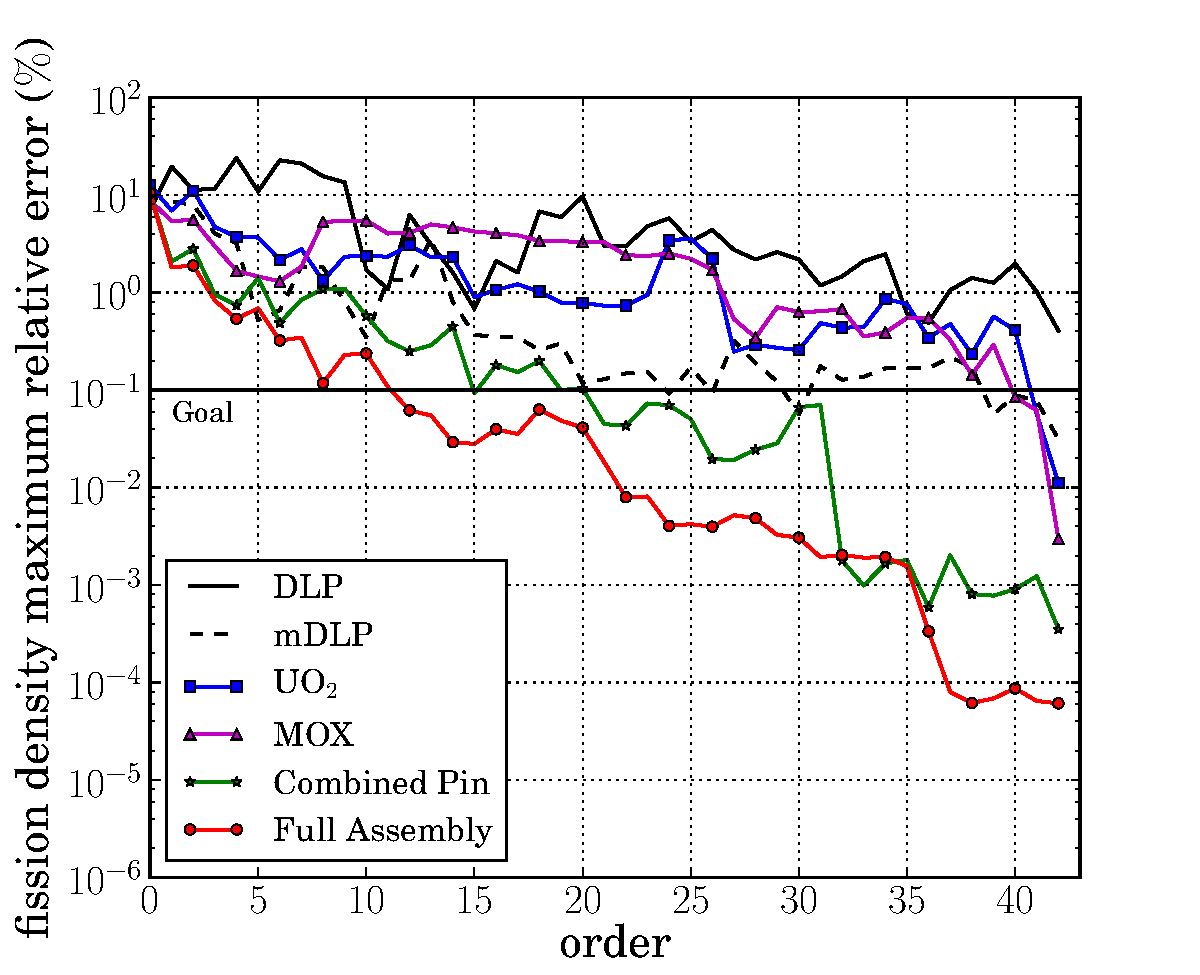
\includegraphics[trim=.1cm .25cm 2.0cm .4cm, clip=true, totalheight=.8\textheight]{10pin_44_energy_basis_comparison_fission-44}
    \end{center}
  \end{frame}

  \begin{frame}
    \frametitle{10-pin 44 g Library}
    \begin{center}
    Using snapshots of $\phi$ and $J_{left}$
    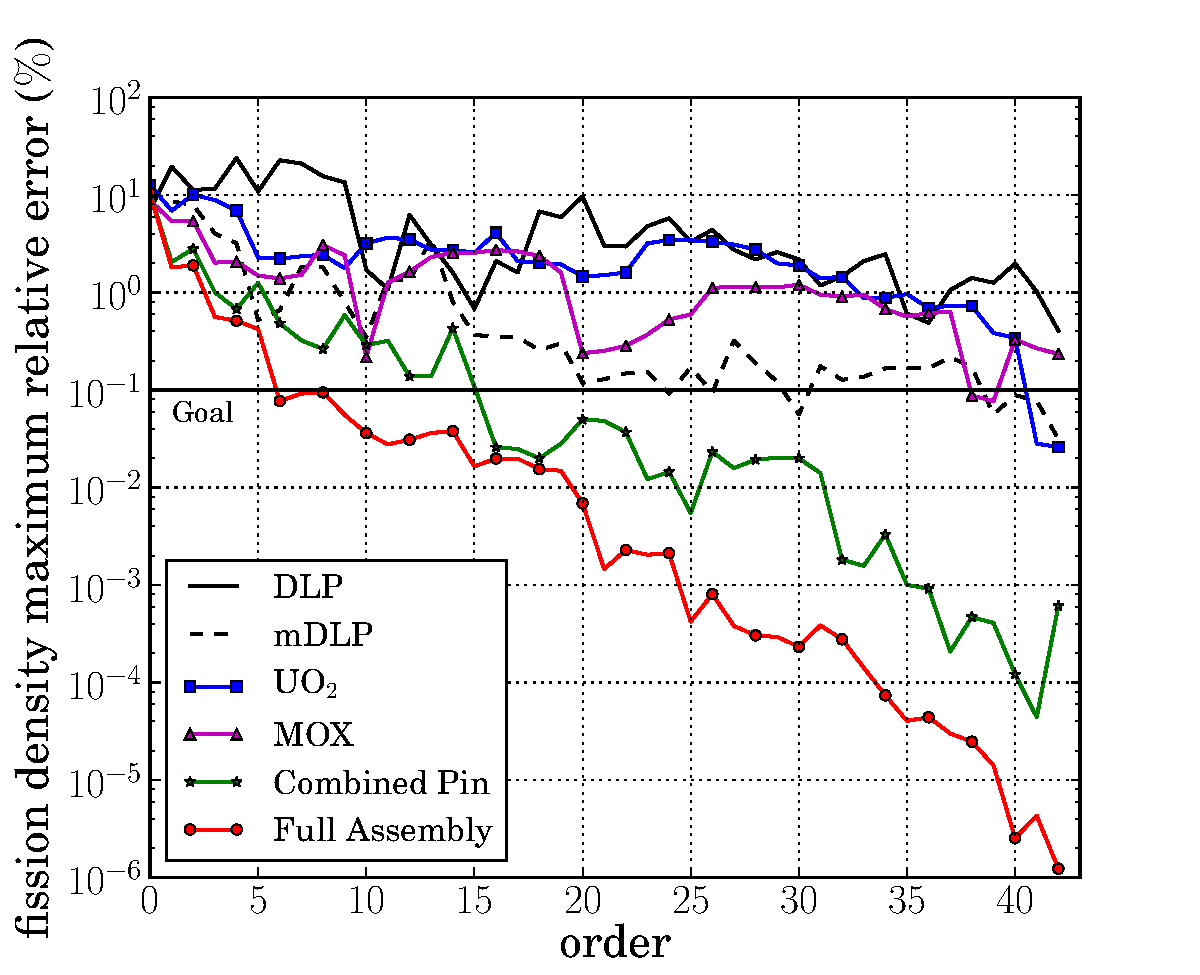
\includegraphics[trim=.1cm .25cm 2.0cm .4cm, clip=true, totalheight=.8\textheight]{10pin_44_partial_energy_basis_comparison_fission-44}
    \end{center}
  \end{frame}

  \begin{frame}
    \frametitle{10-pin 238 g Library}
    \begin{center}
    Using snapshots of only $\phi$
    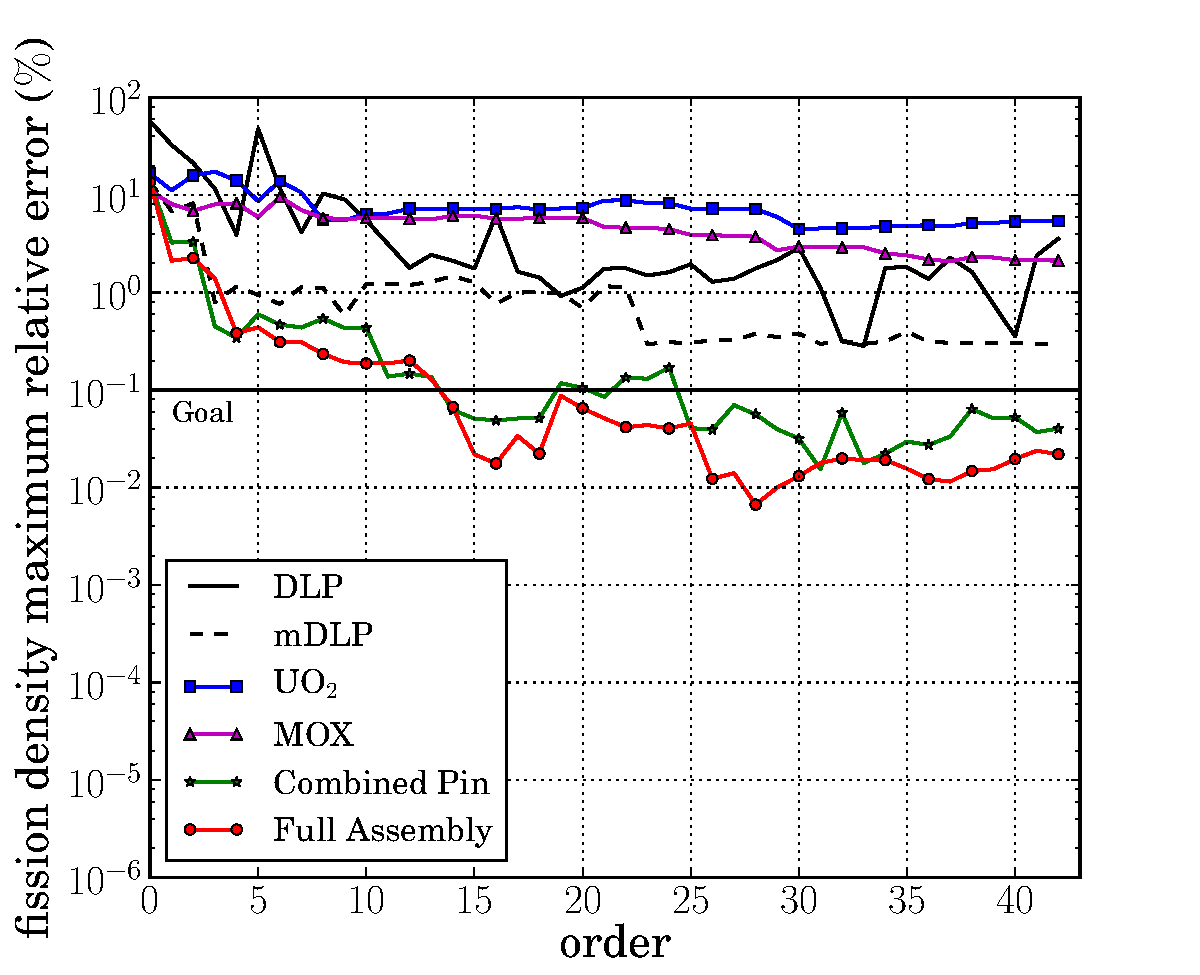
\includegraphics[trim=.1cm .25cm 2.0cm .4cm, clip=true, totalheight=.8\textheight]{10pin_238_energy_basis_comparison_fission-44}
    \end{center}
  \end{frame}

  \begin{frame}
    \frametitle{10-pin 238 g Library}
    \begin{center}
    Using snapshots of $\phi$ and $J_{left}$
    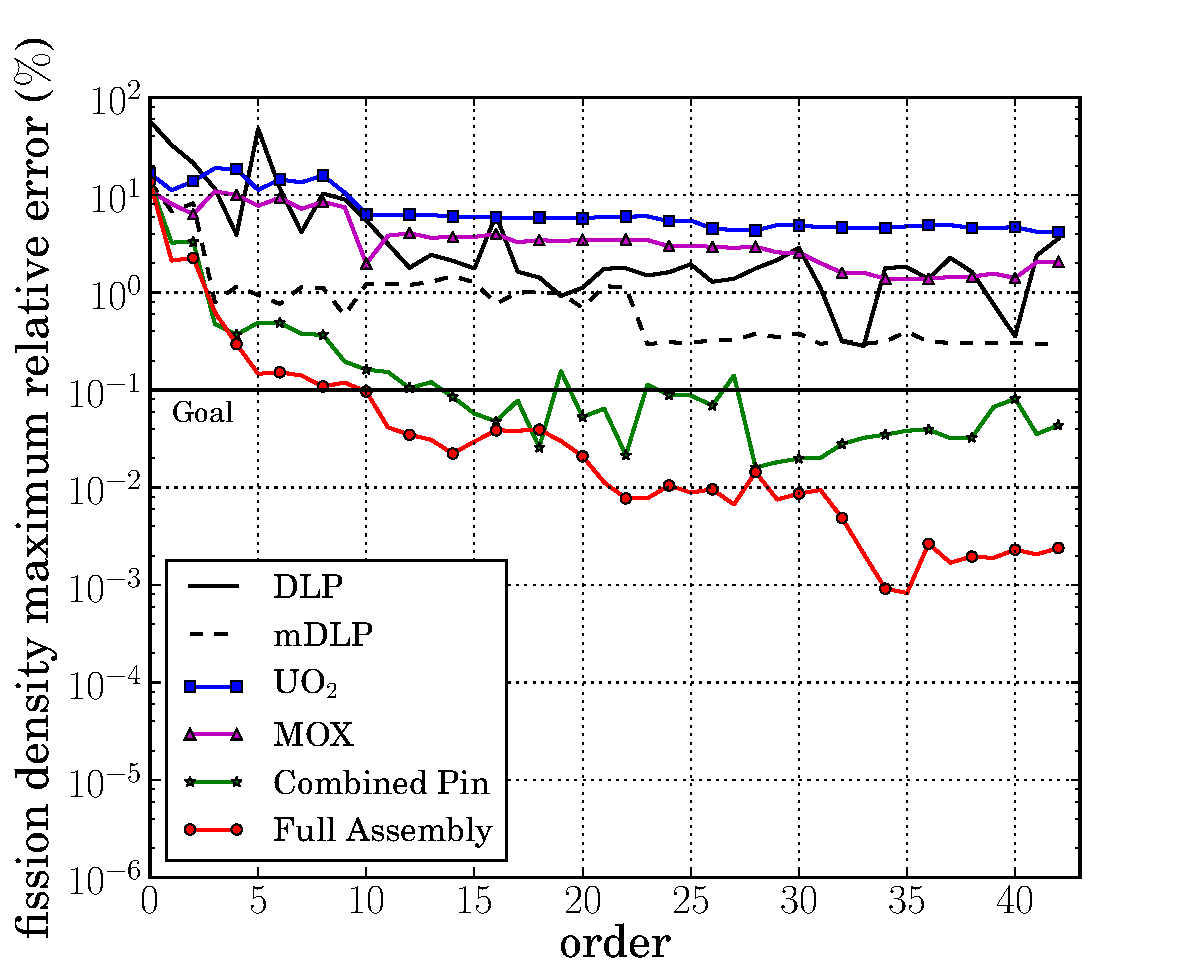
\includegraphics[trim=.1cm .25cm 2.0cm .4cm, clip=true, totalheight=.8\textheight]{10pin_238_partial_energy_basis_comparison_fission-44}
    \end{center}
  \end{frame}

  \begin{frame}
    \frametitle{10-pin 238 g Library}
    \begin{center}
    Adding higher order moments, $0^{th}$ moment is the partial current
    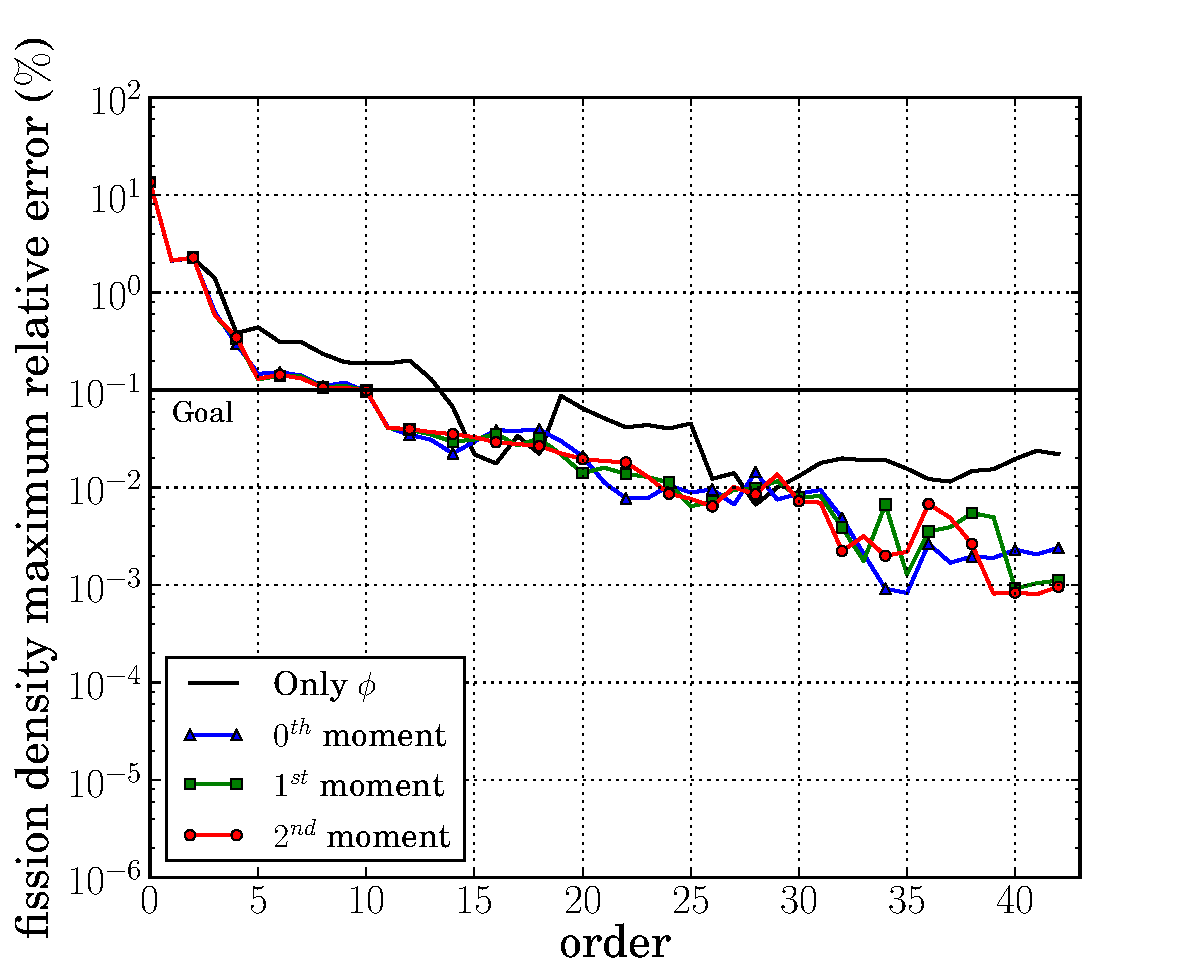
\includegraphics[trim=.1cm .25cm 2.0cm .4cm, clip=true, totalheight=.8\textheight]{10pin_238_angular_comparison_fission_10-pin-44}
    \end{center}
  \end{frame}

  \begin{frame}
    \frametitle{10-pin 238 g Library}
    \begin{center}
    Adding higher order moments, $0^{th}$ moment is the partial current
    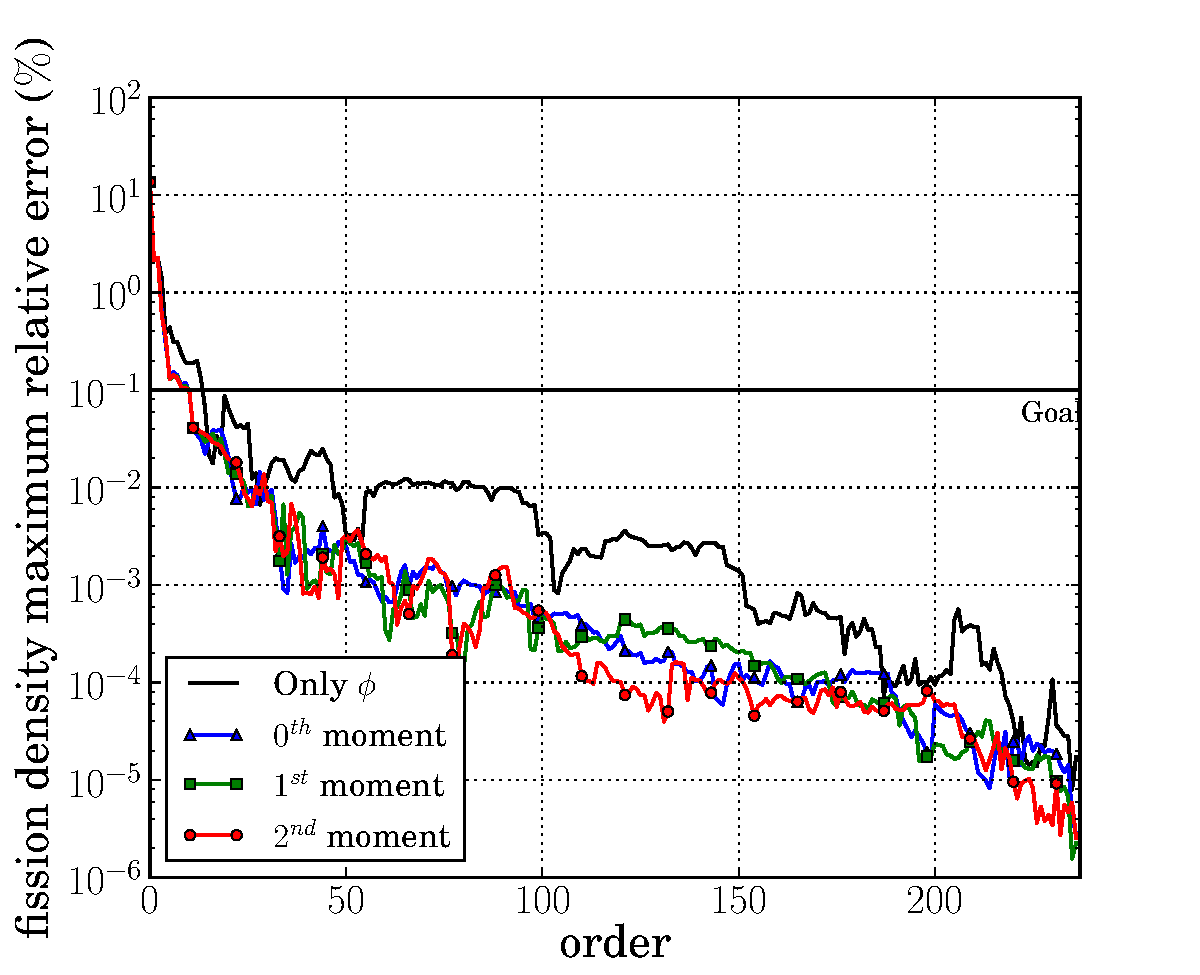
\includegraphics[trim=.1cm .25cm 2.0cm .4cm, clip=true, totalheight=.8\textheight]{10pin_238_angular_comparison_fission_10-pin-238}
    \end{center}
  \end{frame}

%  \begin{frame}
%    \frametitle{Core Configuration 0}
%    \begin{center}
%    Using snapshots of only $\phi$
%    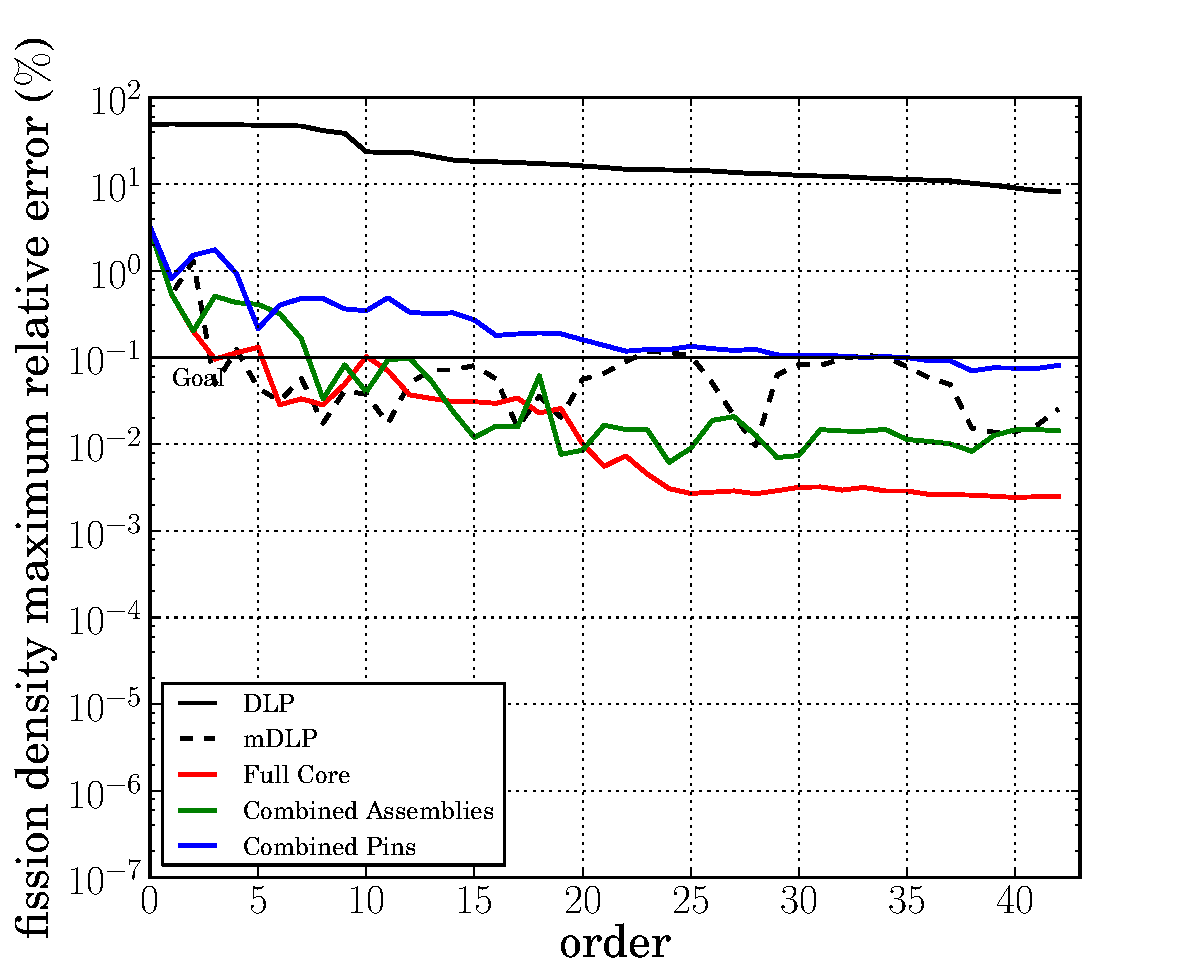
\includegraphics[trim=.1cm .25cm 2.0cm .4cm, clip=true, totalheight=.8\textheight]{core0_energy_basis_comparison_fission-44}
%    \end{center}
%  \end{frame}

%  \begin{frame}
%    \frametitle{Core Configuration 0}
%    \begin{center}
%    Using snapshots of $\phi$ and $J_{left}$
%    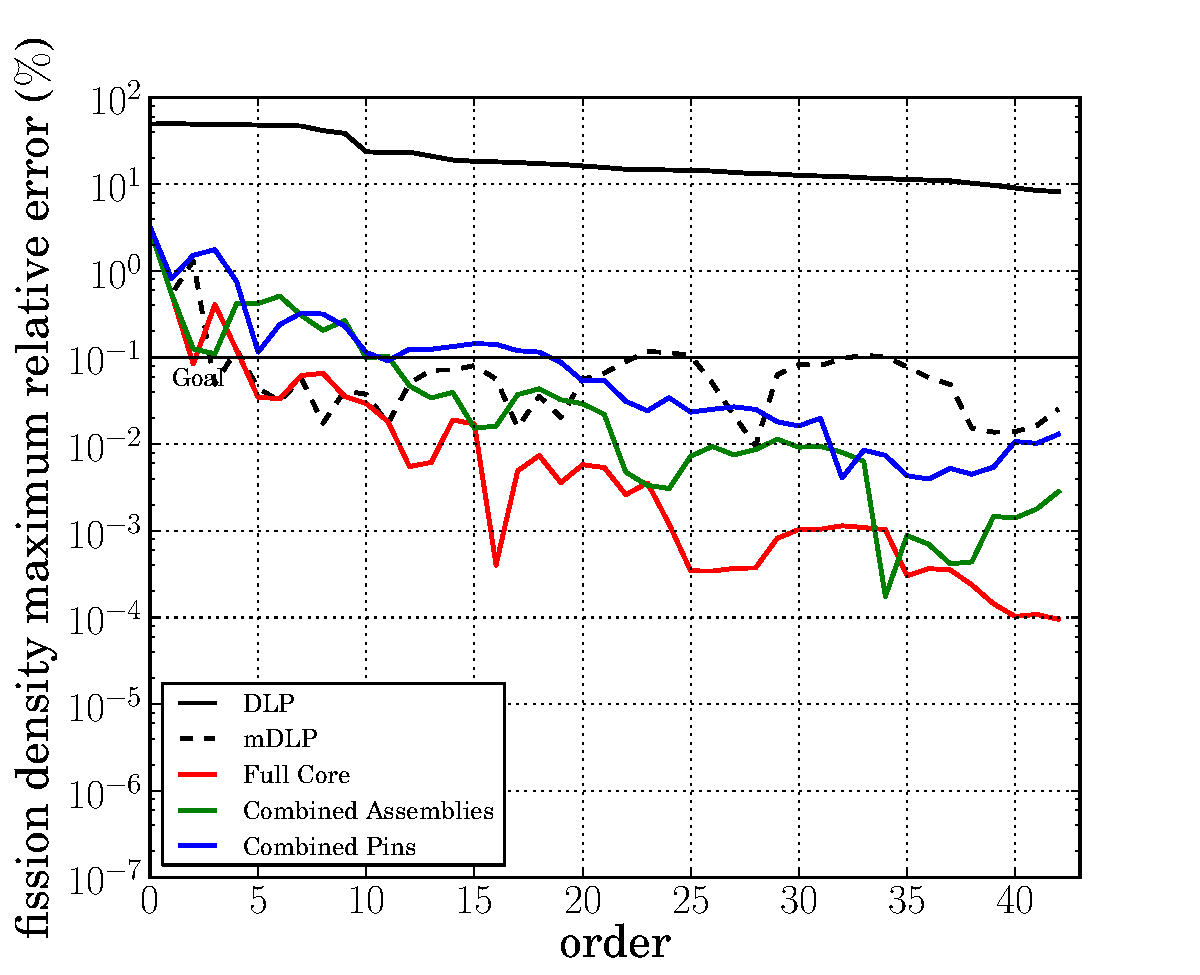
\includegraphics[trim=.1cm .25cm 2.0cm .4cm, clip=true, totalheight=.8\textheight]{core0partial_energy_basis_comparison_fission-44}
%    \end{center}
%  \end{frame}

%  \begin{frame}
%    \frametitle{Core Configuration 1}
%    \begin{center}
%    Using snapshots of only $\phi$
%    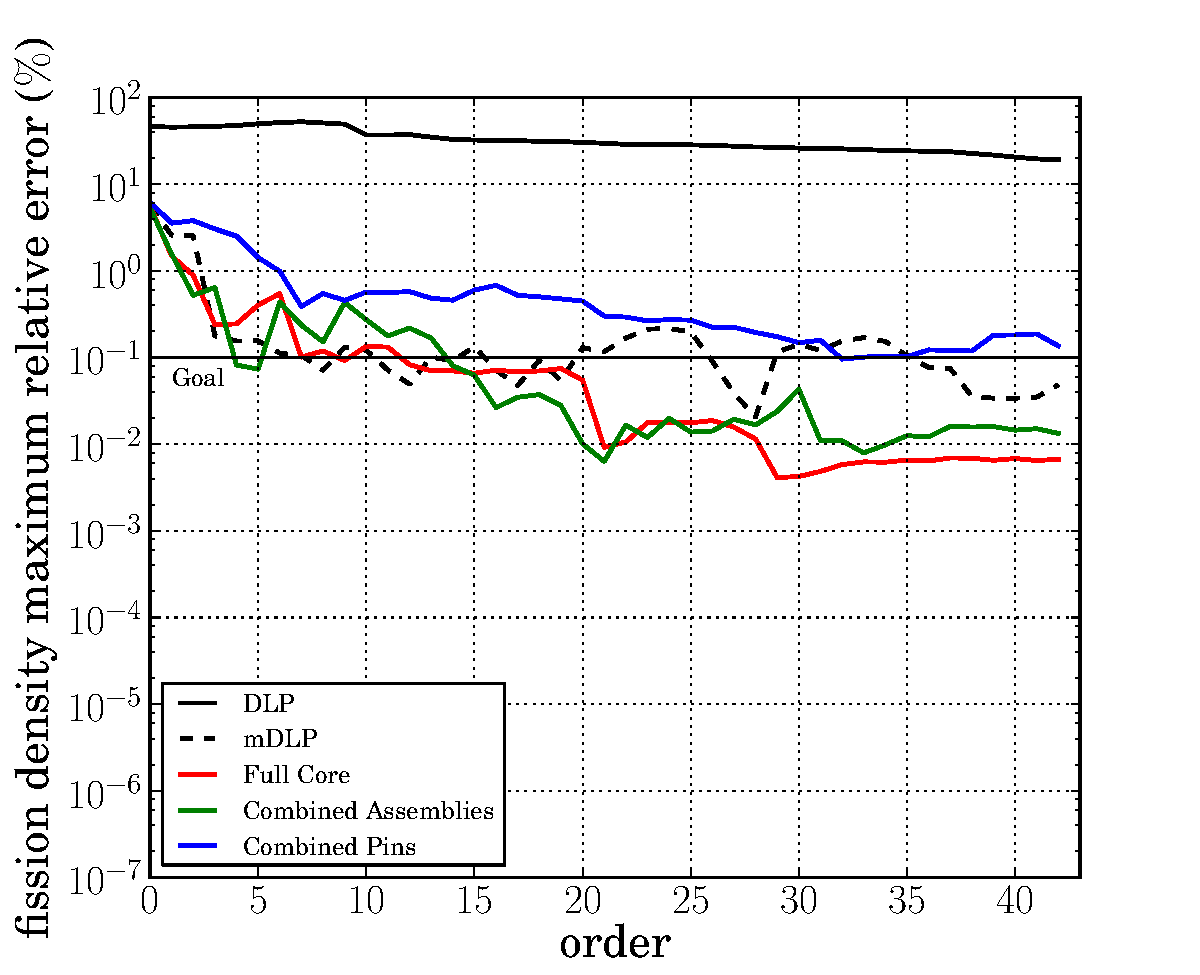
\includegraphics[trim=.1cm .25cm 2.0cm .4cm, clip=true, totalheight=.8\textheight]{core1_energy_basis_comparison_fission-44}
%    \end{center}
%  \end{frame}

%  \begin{frame}
%    \frametitle{Core Configuration 1}
%    \begin{center}
%    Using snapshots of $\phi$ and $J_{left}$
%    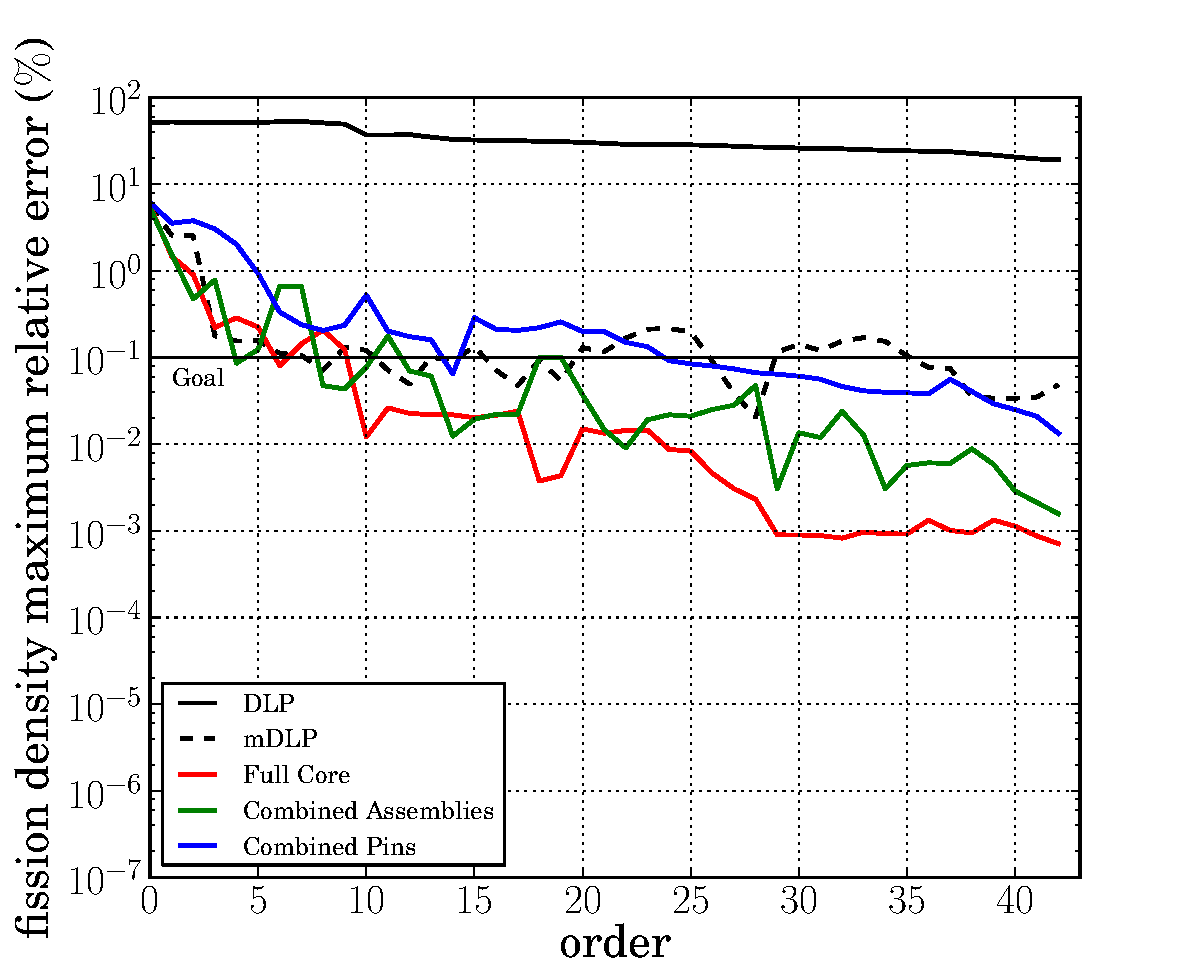
\includegraphics[trim=.1cm .25cm 2.0cm .4cm, clip=true, totalheight=.8\textheight]{core1partial_energy_basis_comparison_fission-44}
%    \end{center}
%  \end{frame}

%  \begin{frame}
%    \frametitle{Core Configuration 2}
%    \begin{center}
%    Using snapshots of only $\phi$
%    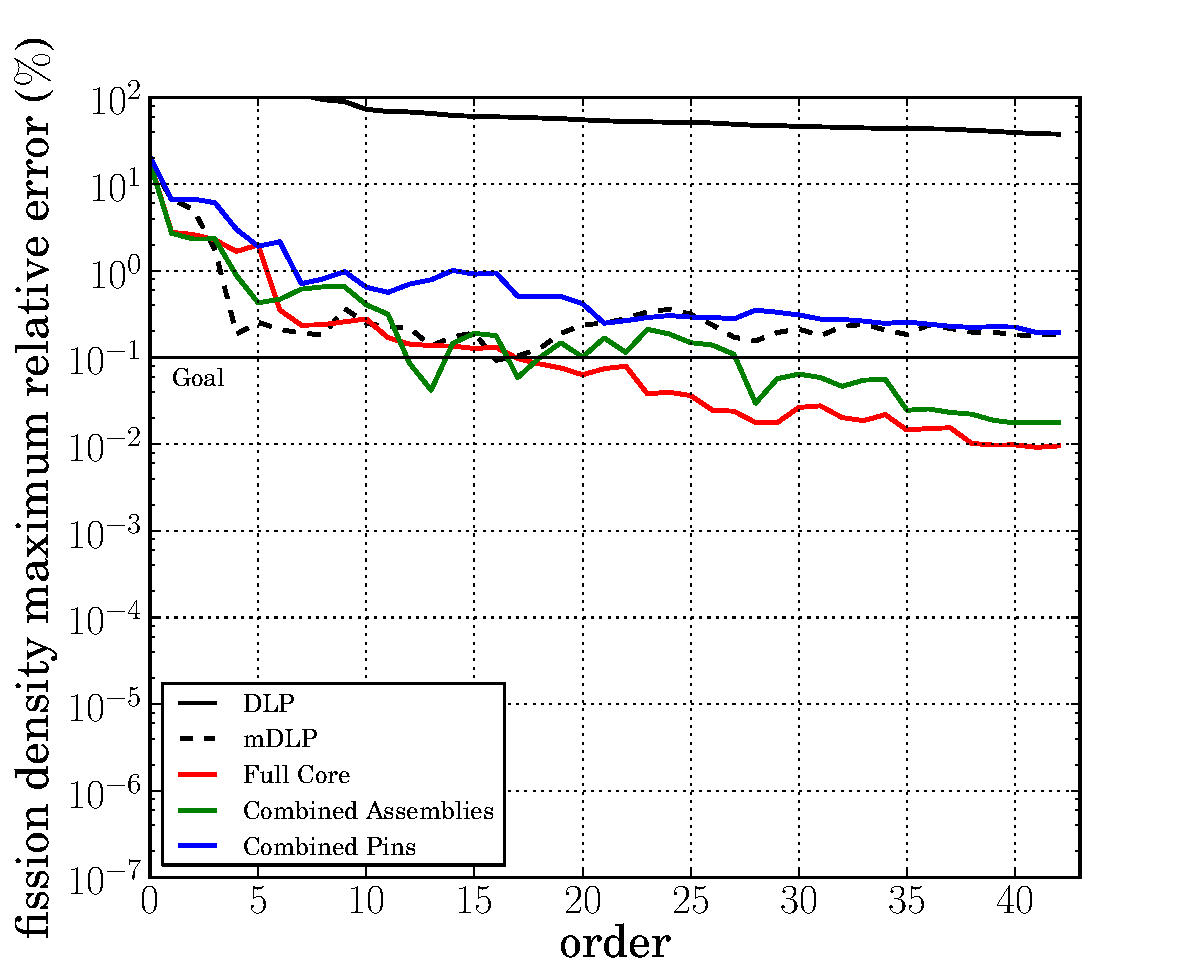
\includegraphics[trim=.1cm .25cm 2.0cm .4cm, clip=true, totalheight=.8\textheight]{core2_energy_basis_comparison_fission-44}
%    \end{center}
%  \end{frame}

%  \begin{frame}
%    \frametitle{Core Configuration 2}
%    \begin{center}
%    Using snapshots of $\phi$ and $J_{left}$
%    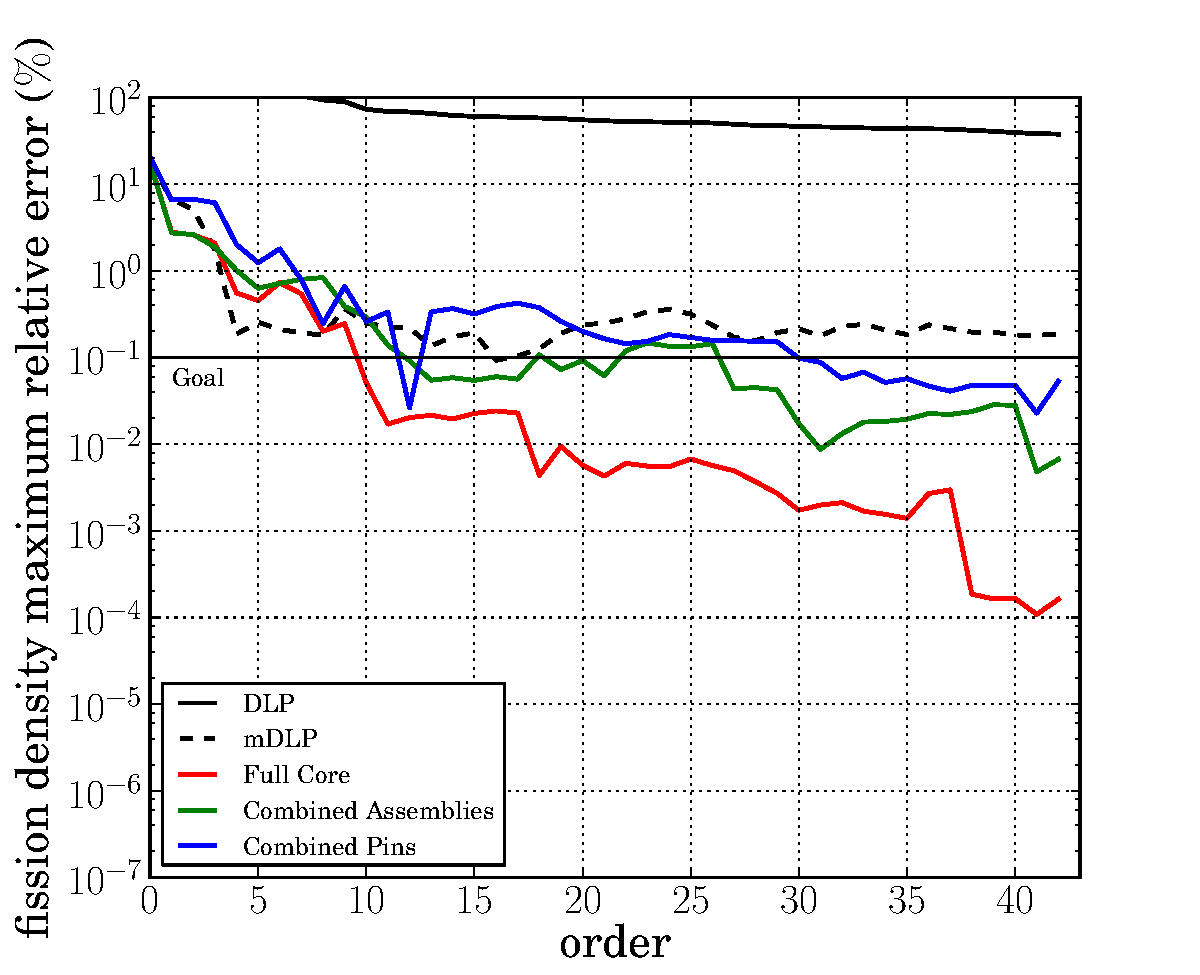
\includegraphics[trim=.1cm .25cm 2.0cm .4cm, clip=true, totalheight=.8\textheight]{core2partial_energy_basis_comparison_fission-44}
%    \end{center}
%  \end{frame}

  \begin{frame}
    \frametitle{BWR Core Comparison}
    \begin{center}
    Using snapshots of only $\phi$. Solid is Core 0, dashed is Core 2.
    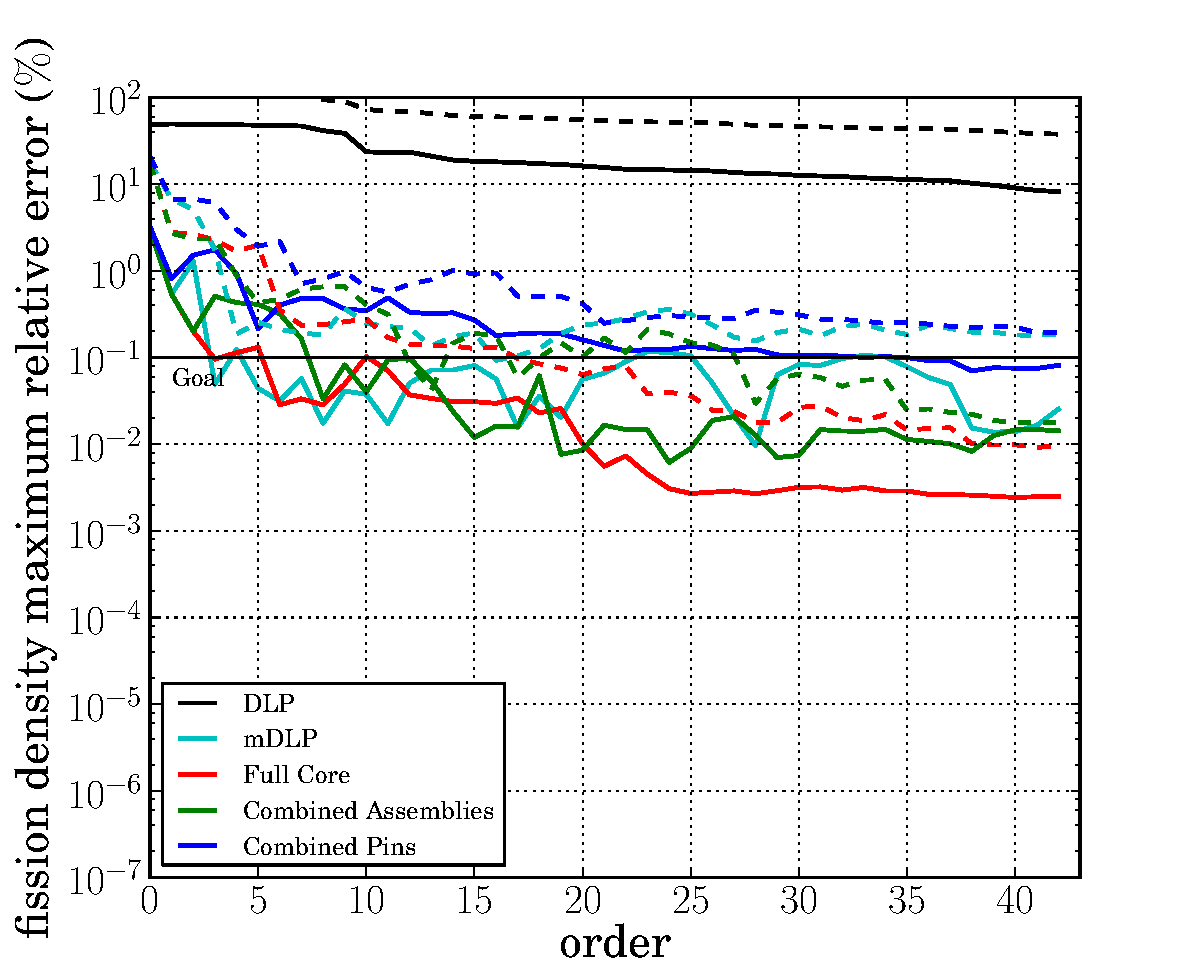
\includegraphics[trim=.1cm .25cm 2.0cm .4cm, clip=true, totalheight=.8\textheight]{BWR_energy_basis_comparison_fission-44}
    \end{center}
  \end{frame}

  \begin{frame}
    \frametitle{BWR Core Comparison}
    \begin{center}
    Using snapshots of $\phi$ and $J_{left}$. Solid is Core 0, dashed is Core 2.
    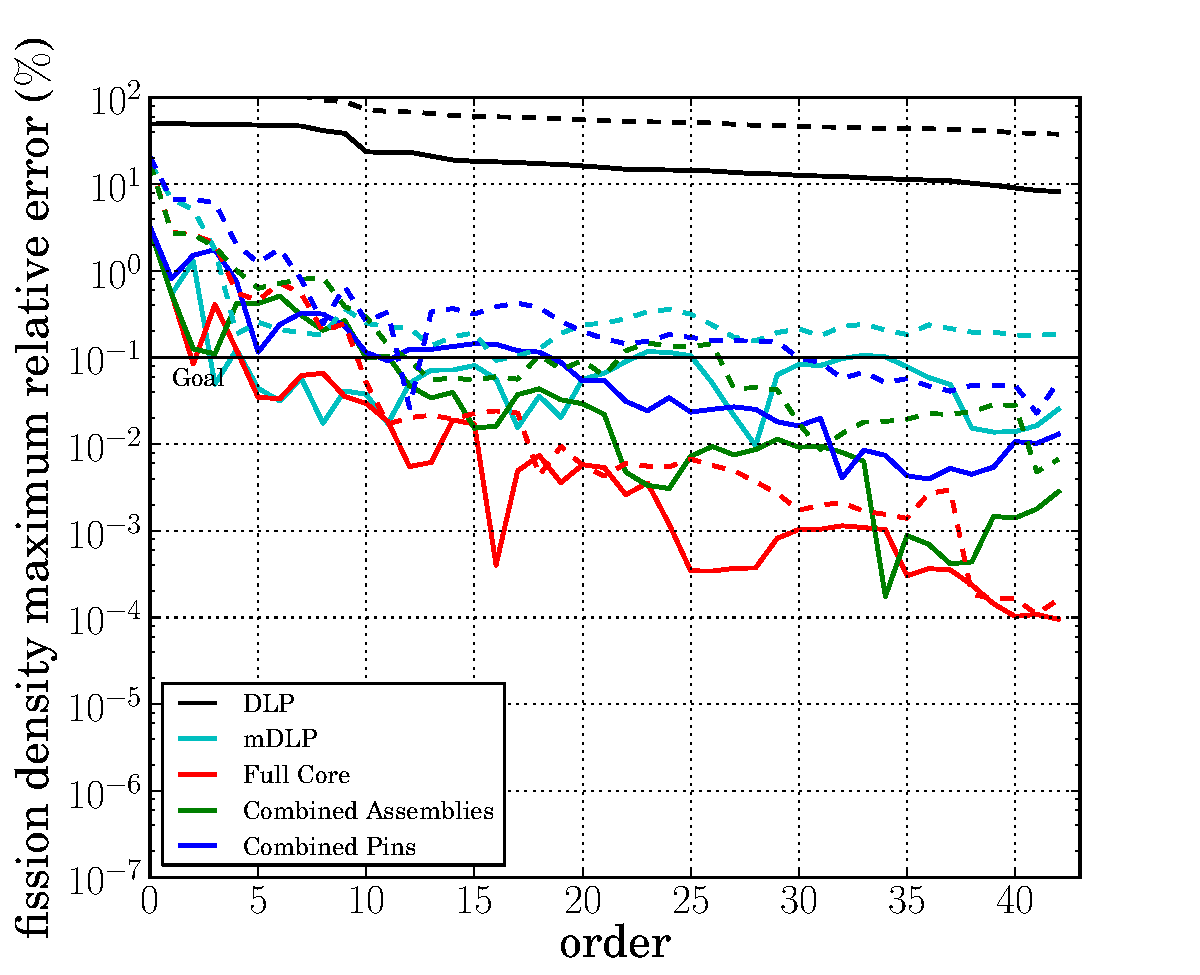
\includegraphics[trim=.1cm .25cm 2.0cm .4cm, clip=true, totalheight=.8\textheight]{BWRpartial_energy_basis_comparison_fission-44}
    \end{center}
  \end{frame}

  \begin{frame}
    \frametitle{BWR Core 0 Angular Moments}
    \begin{center}
    Adding higher order moments, $0^{th}$ moment is the partial current
    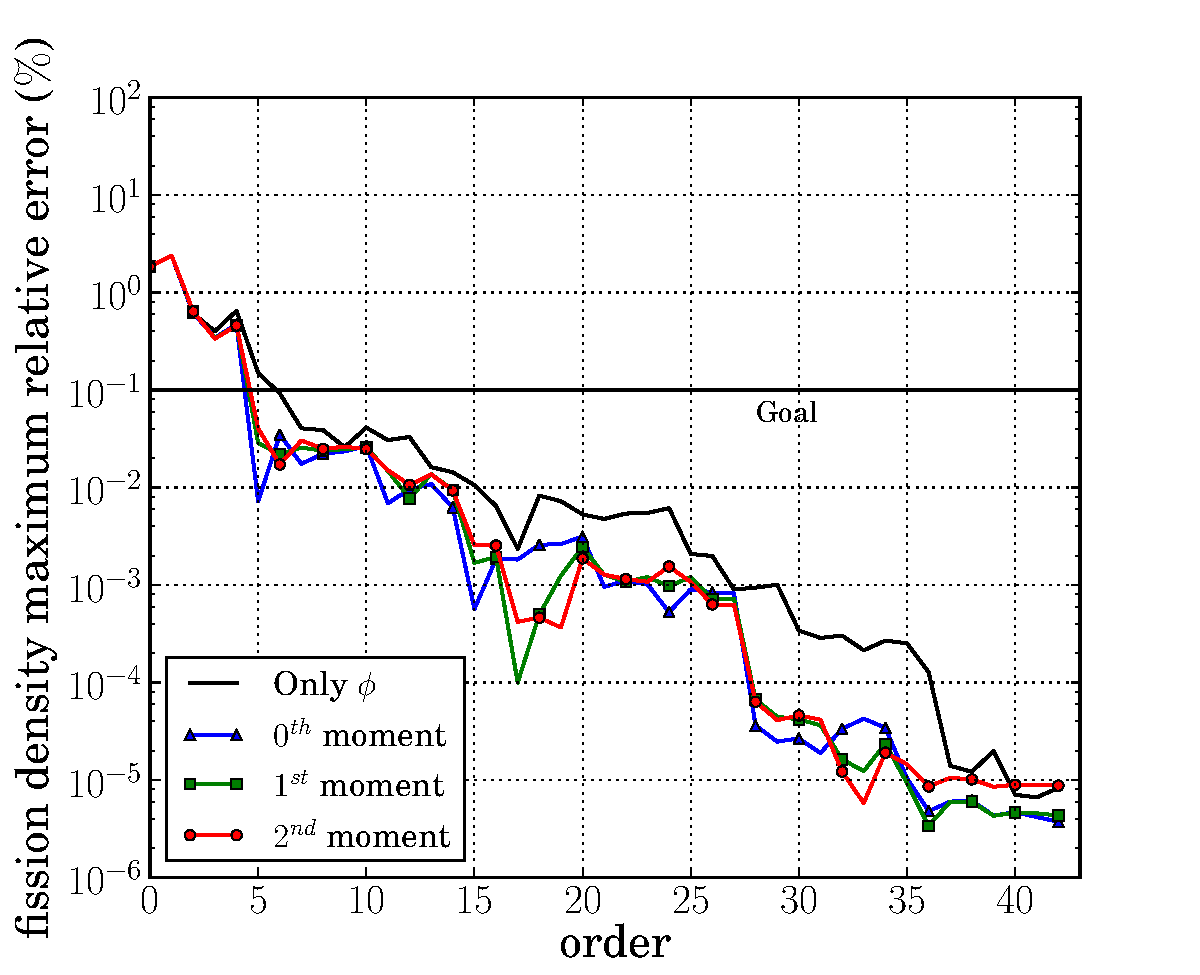
\includegraphics[trim=.1cm .25cm 2.0cm .4cm, clip=true, totalheight=.8\textheight]{BWR0_44_angular_comparison_fission_core-44}
    \end{center}
  \end{frame}

  \begin{frame}
    \frametitle{BWR Core 1 Angular Moments}
    \begin{center}
    Adding higher order moments, $0^{th}$ moment is the partial current
    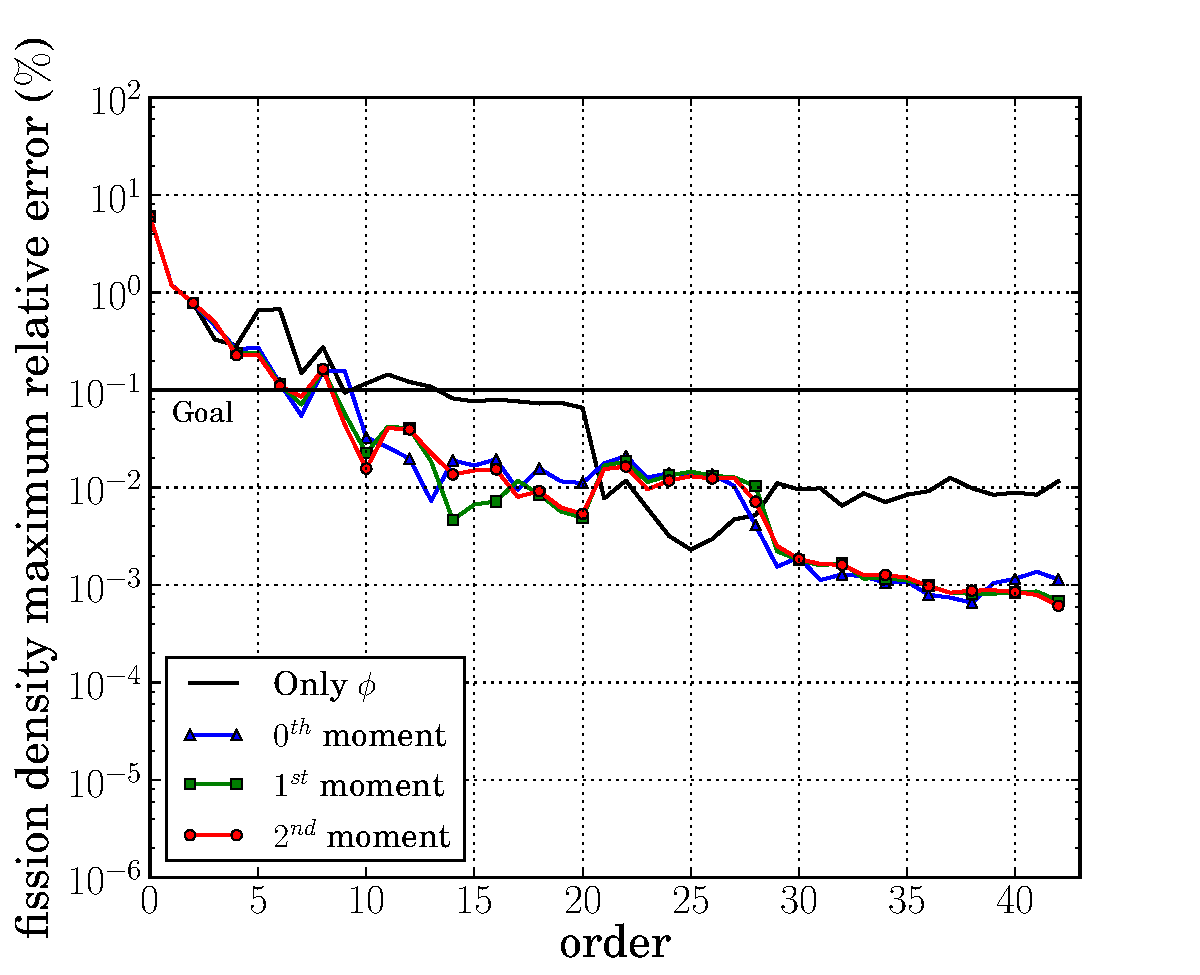
\includegraphics[trim=.1cm .25cm 2.0cm .4cm, clip=true, totalheight=.8\textheight]{BWR1_238_angular_comparison_fission_core-44}
    \end{center}
  \end{frame}

  \begin{frame}
    \frametitle{BWR Core 2 Angular Moments}
    \begin{center}
    Adding higher order moments, $0^{th}$ moment is the partial current
    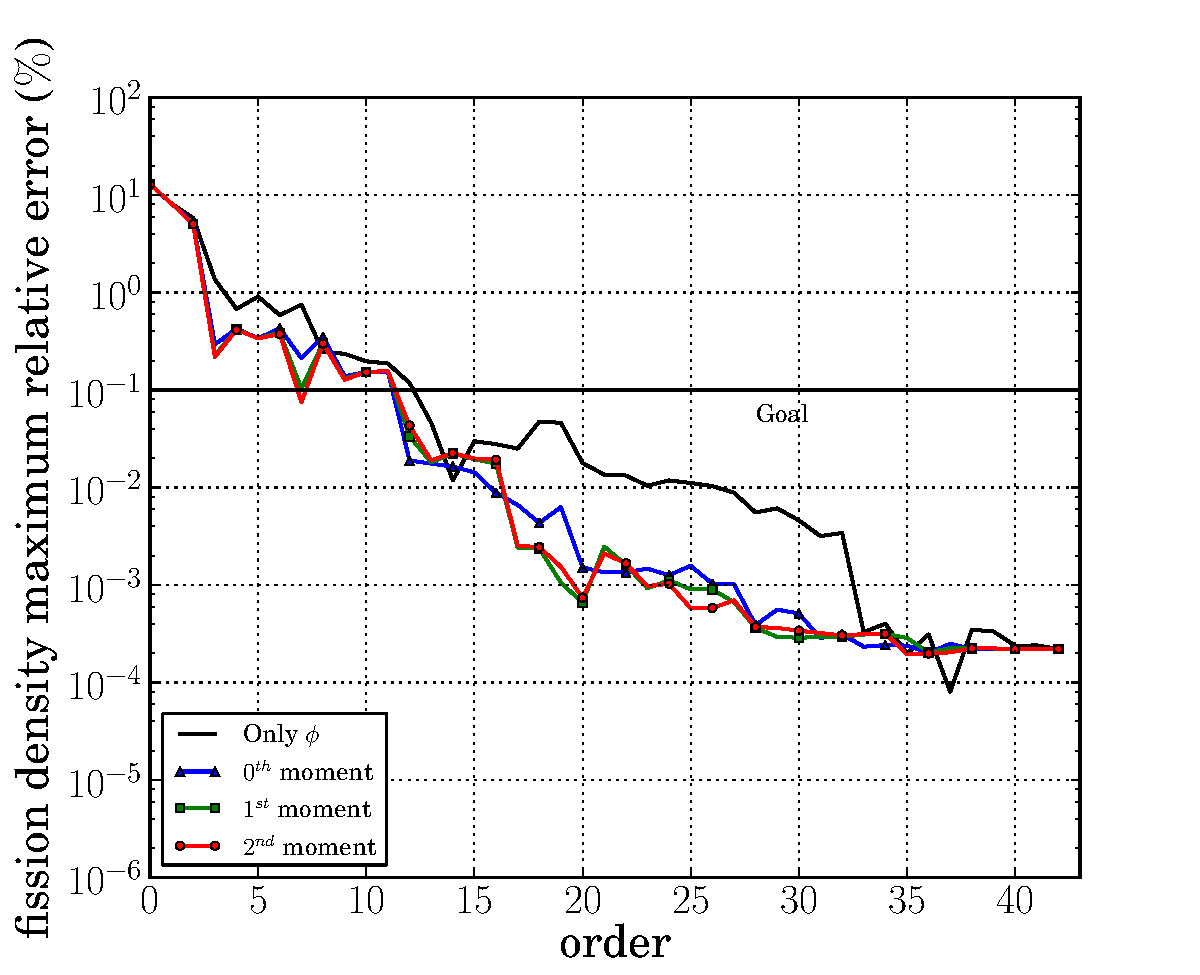
\includegraphics[trim=.1cm .25cm 2.0cm .4cm, clip=true, totalheight=.8\textheight]{BWR2_44_angular_comparison_fission_core-44}
    \end{center}
  \end{frame}

  \section{Conclusion}

  \begin{frame}
    \frametitle{Conclusion}
    \begin{block}{The Karhunen Lo\'{e}ve Transform :}
      \begin{itemize}
	\item Shows improvement over mDLP
	\item Reduces DOF needed for accurate results
	\item Generally improves with increased information
	\item Achieves sub $0.1\%$ error with $<1/10$ DOF
      \end{itemize}
    \end{block}
    \begin{block}{Future Work}
      \begin{itemize}
	\item Expanding to 2D
	\item KLT on spatial variable
	\item Test basis functions using 1 group of snapshots
      \end{itemize}
    \end{block}
    %\begin{block}{Contact Information}
    %  \begin{itemize}
%	\item Richard Reed: blkpawn@k-state.edu
%	\item Dr. Jeremy Roberts: jaroberts@k-state.edu
%      \end{itemize}
%    \end{block}
    \nocite{*}
  \end{frame}

  \begin{frame}[t,allowframebreaks]\label{lastframe}
    \frametitle{References}
    \bibliographystyle{ans}
    \bibliography{bibliography}
  \end{frame}

  \beginbackup

  \begin{frame}[noframenumbering]
    \frametitle{10-pin 238 g Library}
    \begin{center}
    Using snapshots of only $\phi$
    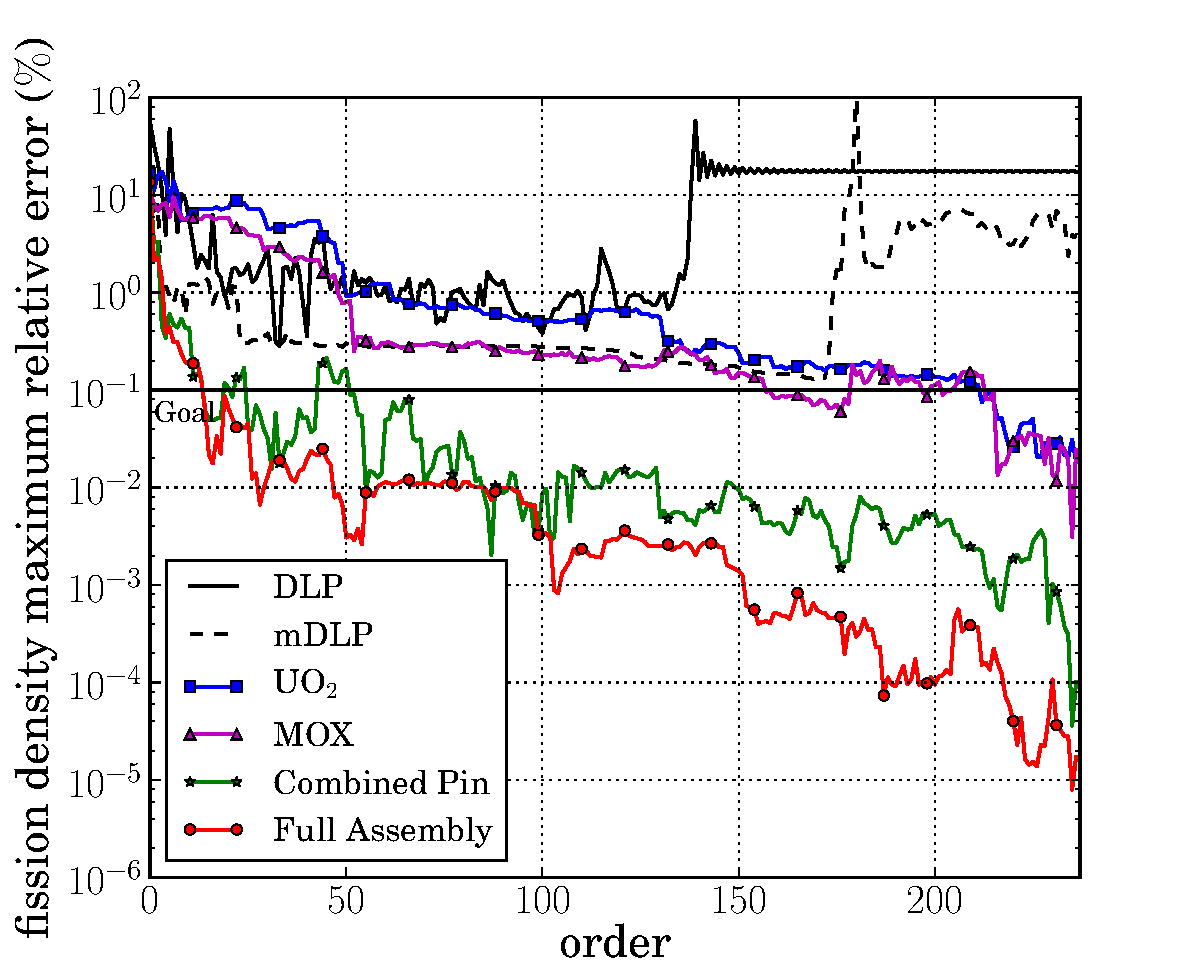
\includegraphics[trim=.1cm .25cm 2.0cm .4cm, clip=true, totalheight=.8\textheight]{10pin_238_energy_basis_comparison_fission-238}
    \end{center}
  \end{frame}

  \begin{frame}[noframenumbering]
    \frametitle{10-pin 238 g Library}
    \begin{center}
    Using snapshots of $\phi$ and $J_{left}$
    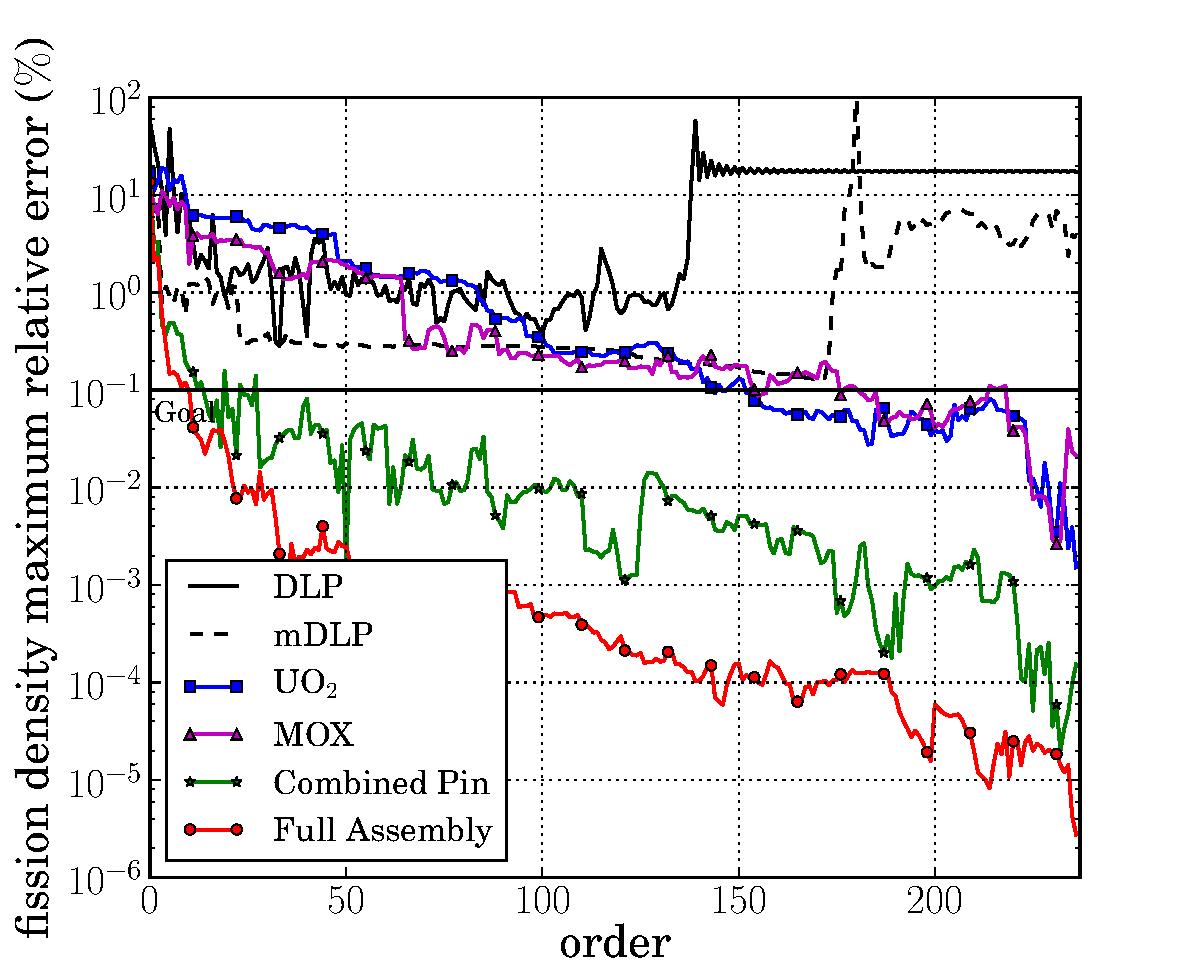
\includegraphics[trim=.1cm .25cm 2.0cm .4cm, clip=true, totalheight=.8\textheight]{10pin_238_partial_energy_basis_comparison_fission-238}
    \end{center}
  \end{frame}

%  \begin{frame}[noframenumbering]
%    \frametitle{Core Configuration 0}
%    \begin{center}
%    Using snapshots of only $\phi$
%    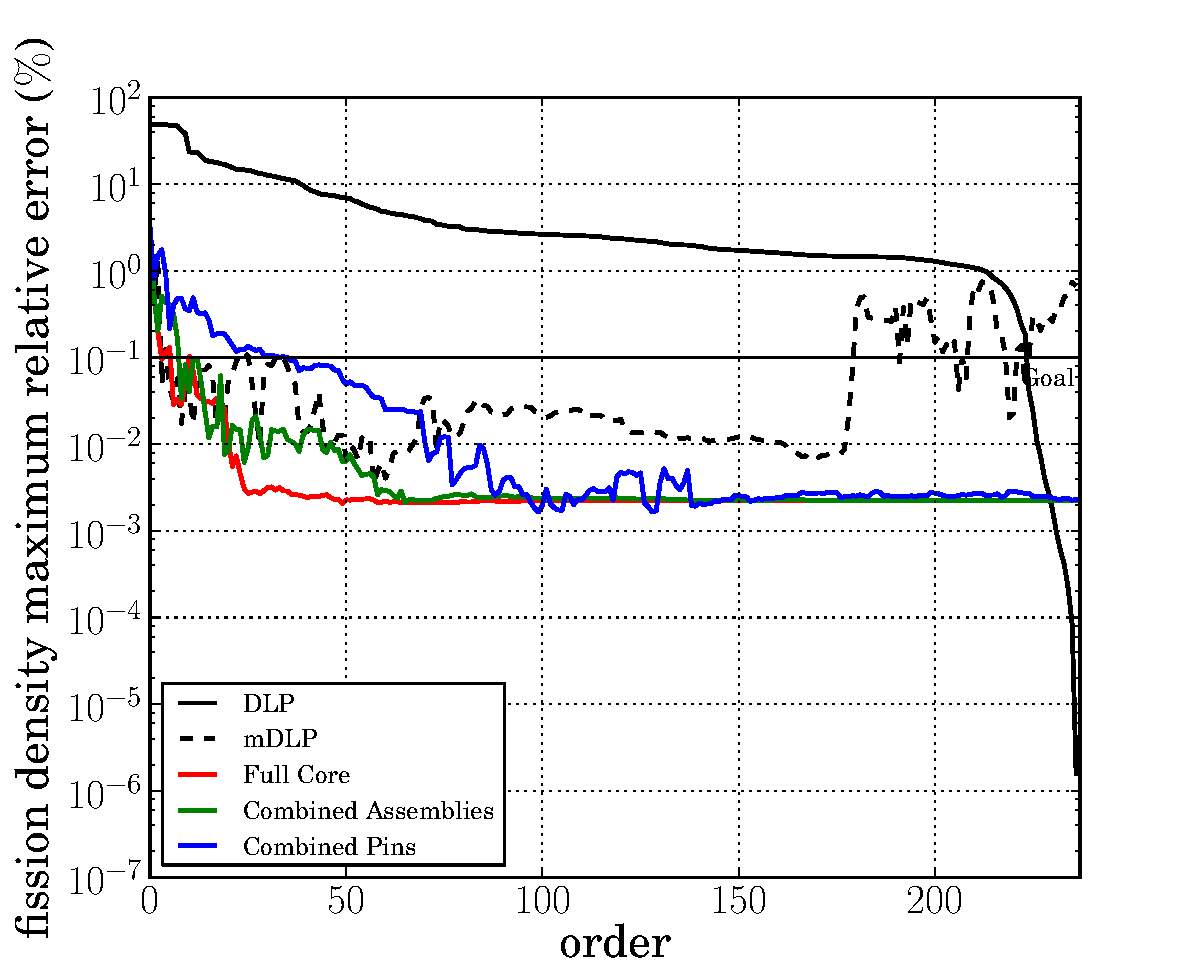
\includegraphics[trim=.1cm .25cm 2.0cm .4cm, clip=true, totalheight=.8\textheight]{core0_energy_basis_comparison_fission-238}
%    \end{center}
%  \end{frame}

%  \begin{frame}[noframenumbering]
%    \frametitle{Core Configuration 0}
%    \begin{center}
%    Using snapshots of $\phi$ and $J_{left}$
%    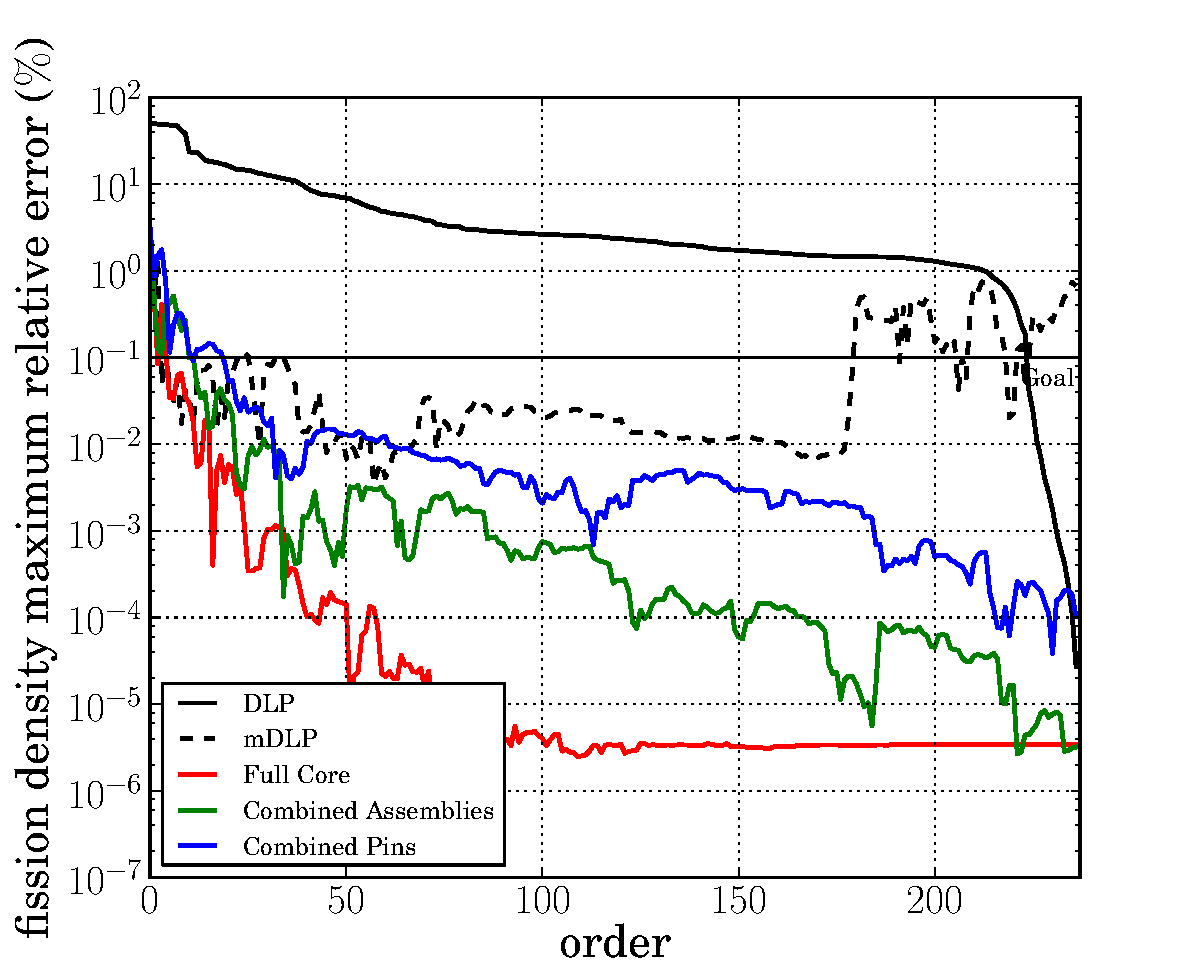
\includegraphics[trim=.1cm .25cm 2.0cm .4cm, clip=true, totalheight=.8\textheight]{core0partial_energy_basis_comparison_fission-238}
%    \end{center}
%  \end{frame}

%  \begin{frame}[noframenumbering]
%    \frametitle{Core Configuration 1}
%    \begin{center}
%    Using snapshots of only $\phi$
%    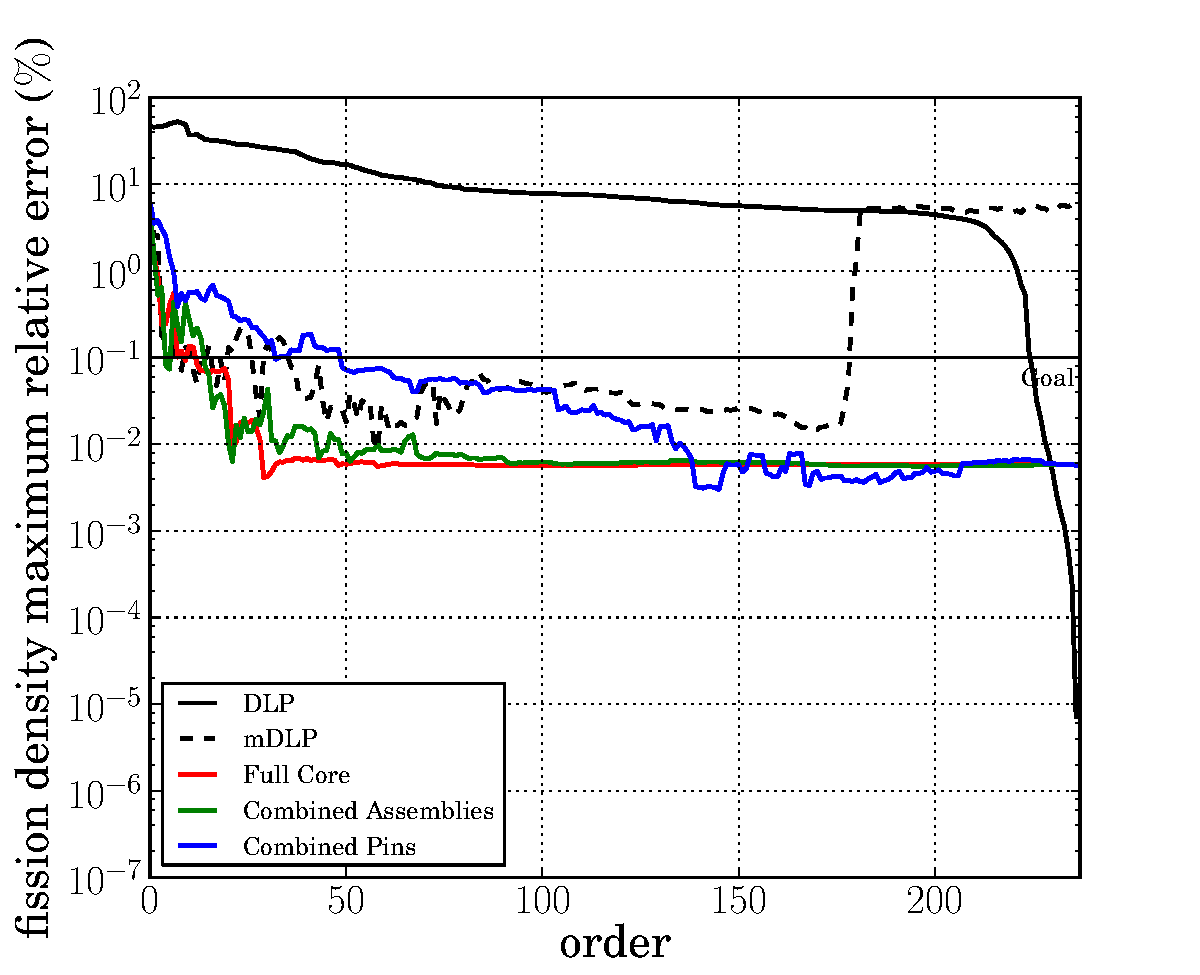
\includegraphics[trim=.1cm .25cm 2.0cm .4cm, clip=true, totalheight=.8\textheight]{core1_energy_basis_comparison_fission-238}
%    \end{center}
%  \end{frame}

%  \begin{frame}[noframenumbering]
%    \frametitle{Core Configuration 1}
%    \begin{center}
%    Using snapshots of $\phi$ and $J_{left}$
%    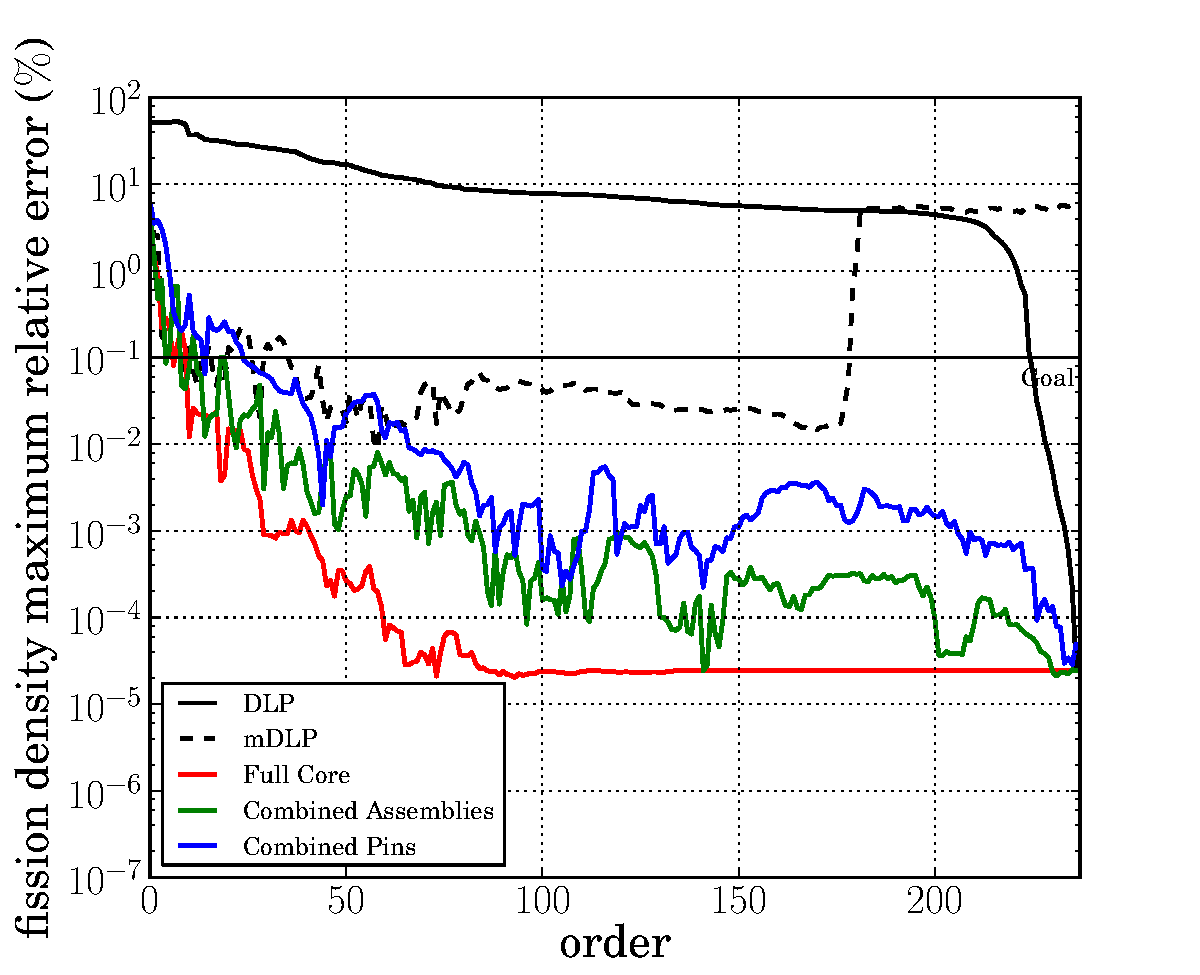
\includegraphics[trim=.1cm .25cm 2.0cm .4cm, clip=true, totalheight=.8\textheight]{core1partial_energy_basis_comparison_fission-238}
%    \end{center}
%  \end{frame}

%  \begin{frame}[noframenumbering]
%    \frametitle{Core Configuration 2}
%    \begin{center}
%    Using snapshots of only $\phi$
%    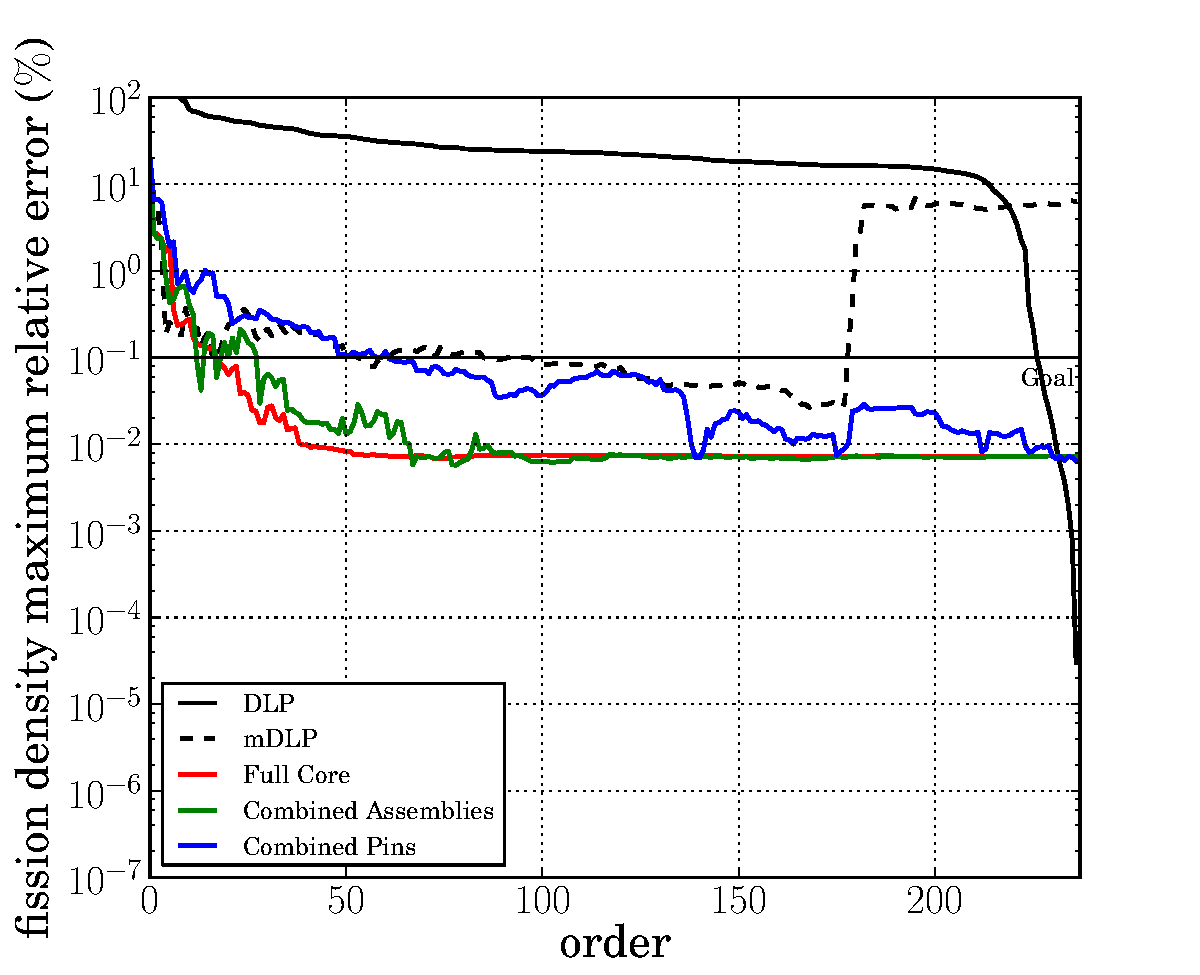
\includegraphics[trim=.1cm .25cm 2.0cm .4cm, clip=true, totalheight=.8\textheight]{core2_energy_basis_comparison_fission-238}
%    \end{center}
%  \end{frame}

%  \begin{frame}[noframenumbering]
%    \frametitle{Core Configuration 2}
%    \begin{center}
%    Using snapshots of $\phi$ and $J_{left}$
%    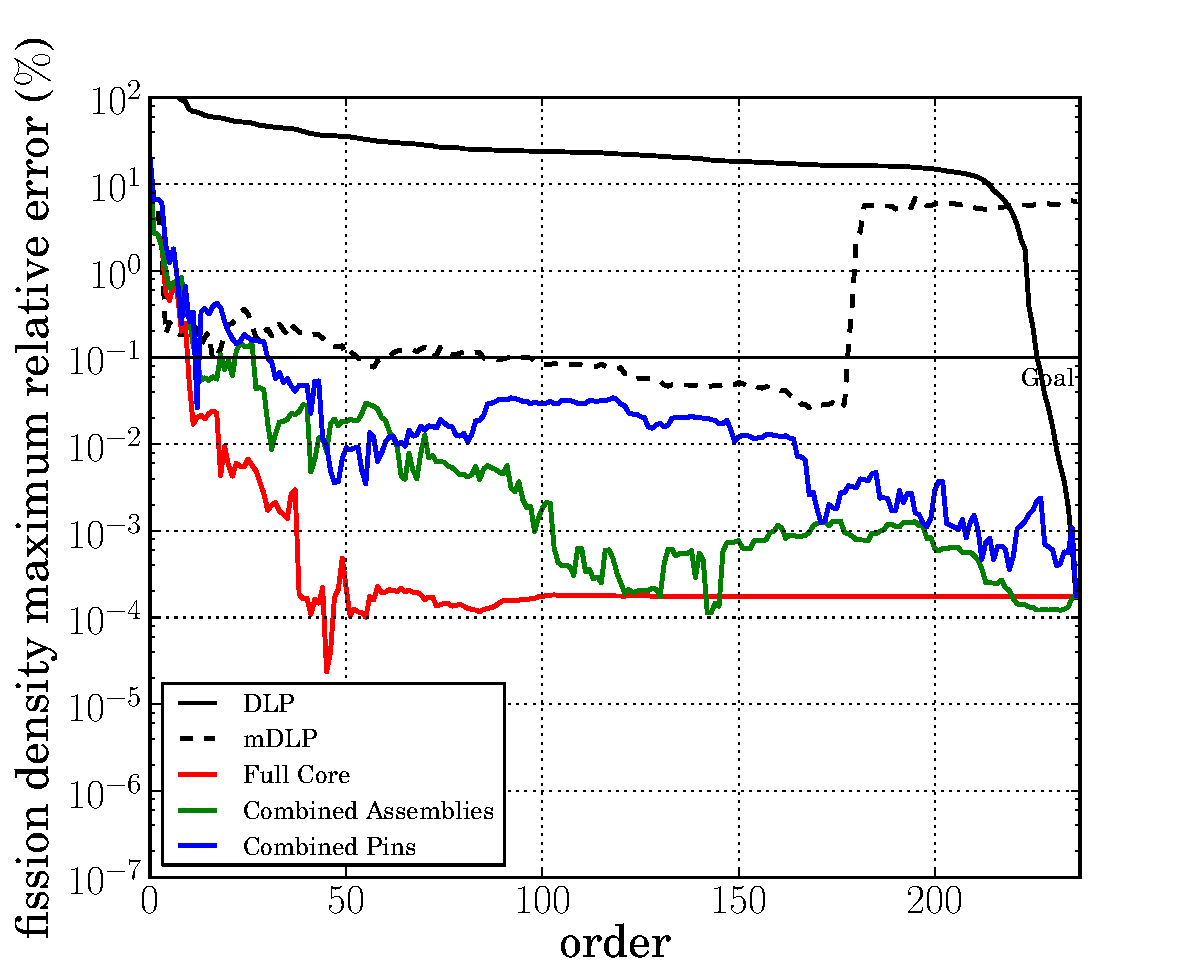
\includegraphics[trim=.1cm .25cm 2.0cm .4cm, clip=true, totalheight=.8\textheight]{core2partial_energy_basis_comparison_fission-238}
%    \end{center}
%  \end{frame}

  \begin{frame}[noframenumbering]
    \frametitle{BWR Core Comparison}
    \begin{center}
    Using snapshots of only $\phi$
    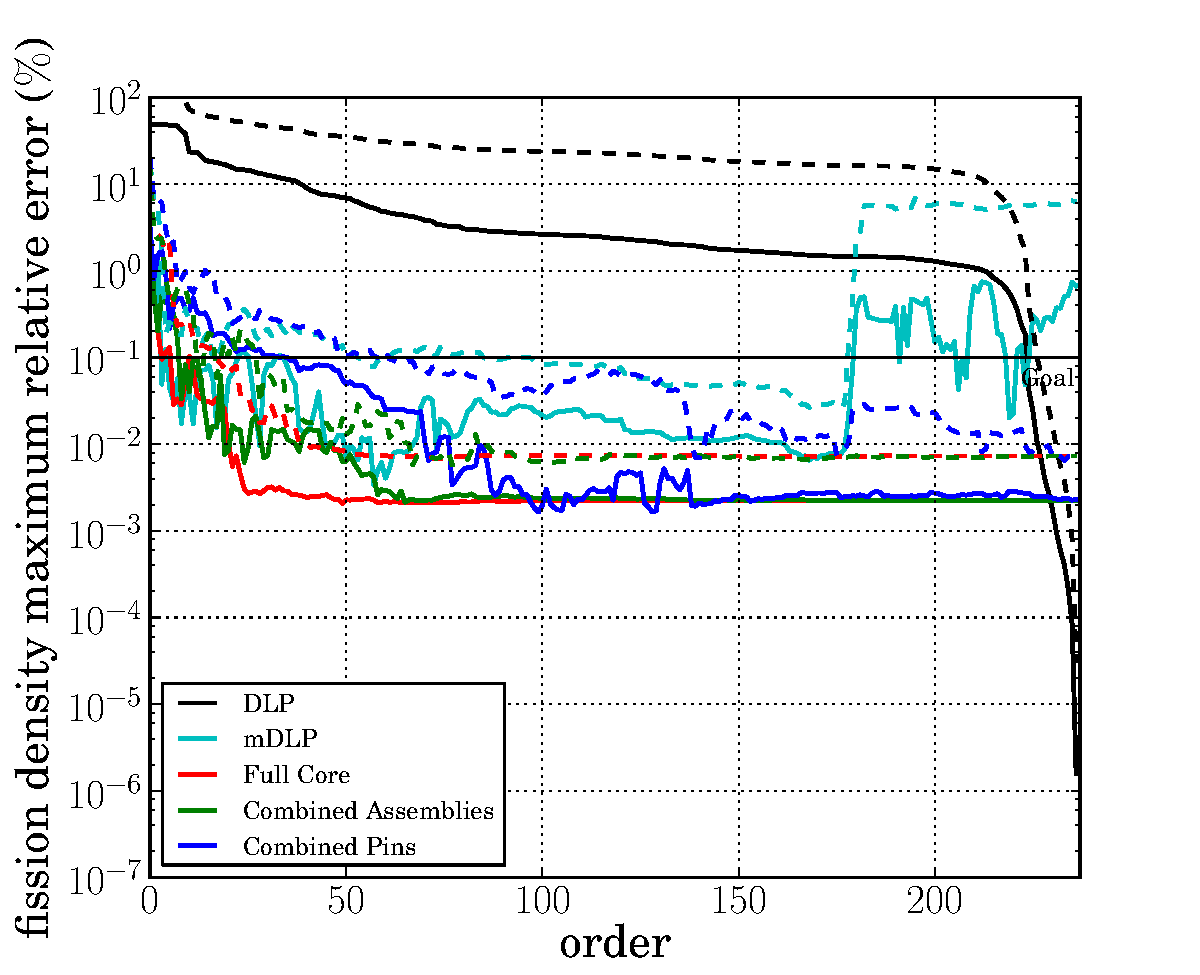
\includegraphics[trim=.1cm .25cm 2.0cm .4cm, clip=true, totalheight=.8\textheight]{BWR_energy_basis_comparison_fission-238}
    \end{center}
  \end{frame}

  \begin{frame}[noframenumbering]
    \frametitle{BWR Core Comparison}
    \begin{center}
    Using snapshots of $\phi$ and $J_{left}$
    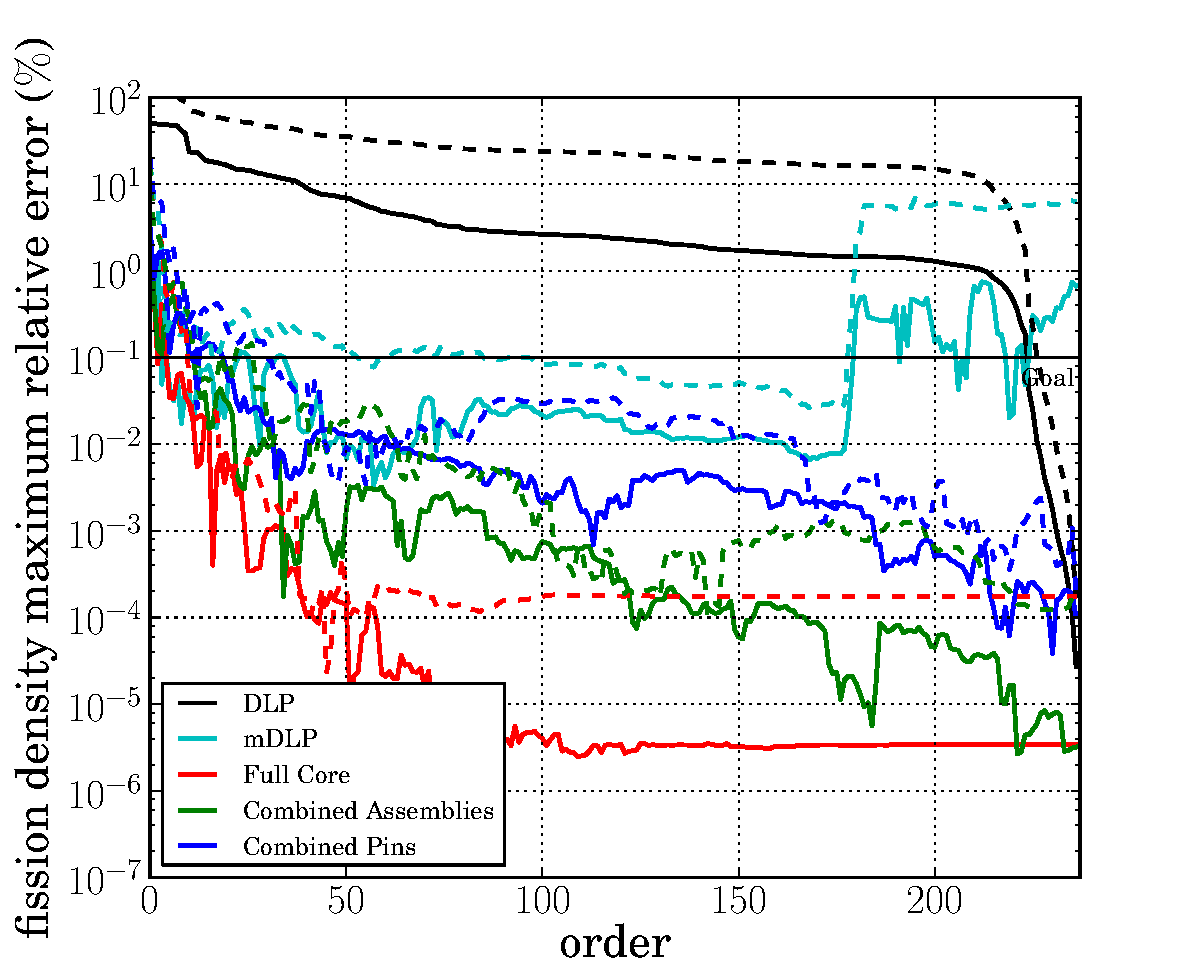
\includegraphics[trim=.1cm .25cm 2.0cm .4cm, clip=true, totalheight=.8\textheight]{BWRpartial_energy_basis_comparison_fission-238}
    \end{center}
  \end{frame}

  \backupend

\end{document}
